\documentclass[a4paper,twoside,11pt,reqno]{mwrep}
\usepackage[utf8]{inputenc}
\usepackage{polski}
\usepackage[table]{xcolor}%dodane
\usepackage{graphicx}
%%%%%%%%%%%%%%%%%%%%%%%%%%%%
% pakiety matematyczne
\usepackage{amsmath}
\usepackage{amsthm}
\usepackage{amssymb}
\usepackage{enumerate}
\usepackage{hyperref}
%%%%%%%%%%%%%%%%%%%%%%%%%%%%
%%%%%%%%%%%%%%%%%%%%%%%%%%%%
% Ustawienia wymiarów strony
\usepackage{geometry}
 \geometry{
    paper=a4paper,
    inner=30mm,         % Inner margin
    outer=20mm,         % Outer margin
    %bindingoffset=10mm, % Binding offset
    nohead,
    top=20mm,           % Top margin
    bottom=25mm,        % Bottom margin
    }
%%%%%%%%%%%%%%%%%%%%%%%%%%%
% komenda dodająca pustą stronę
\newcommand\blankpage{%
    \null
    \thispagestyle{empty}%
    \addtocounter{page}{-1}%
    \newpage}
%%%%%%%%%%%%%%%%%%%%%%%%%%
% wprowadzenie środowisk dla twierdzeń, lematów, definicji i wnisoków
% Uwaga: można zastosować własne nazwy w miejsce thm, lem, defn i rem
\theoremstyle{plain} \newtheorem{twr}{Twierdzenie}
\theoremstyle{plain} \newtheorem{lem}{Lemat}
\theoremstyle{definition} \newtheorem{defi}{Definicja}
\theoremstyle{remark} \newtheorem*{wni}{Wniosek}
\theoremstyle{definition} \newtheorem{uwaga}{Uwaga}
\theoremstyle{definition}\newtheorem{prz}{Przykład}
\newenvironment{dowod}{\par\vspace{0.1cm}\par{\sc Dowód.}}{\hfill $\blacksquare$\par\vspace{0.4cm}\par}
%%%%%%%%%%%%%%%%%%%%%%%%%%%%%%%%%%%%%%%%%%%%%%%%%%%%%%%%%%%%%%%%
% Informacje na stronę tytułową
\newcommand{\autor}{\fontfamily{qhv}\fontshape{sf}\selectfont\LARGE\bfseries
Szymon Sroka} % Wpisz swoje imię i nazwisko
%
\newcommand{\album}{\fontfamily{qhv}\fontshape{sf}\selectfont
130471}% Wpisz swój numer albumu
%
\newcommand{\pltitle}{\fontfamily{qhv}\fontshape{sf}\selectfont\LARGE\bfseries
Kwaterniony, obroty i animacje komputerowe} % Wpisz tytuł swojej pracy po polsku
%
\newcommand{\engtitle}{\fontfamily{qhv}\fontshape{sf}\selectfont\LARGE\bfseries
Selected theorems on linear capacity of matrix sets} %  Wpisz tytuł swojej pracy po angielsku
%
\newcommand{\level}{\fontfamily{qhv}\fontshape{sf}\selectfont\large
magisterska} % Wybierz odpowiednie określenie
%
\newcommand{\promotor}{\fontfamily{qhv}\fontshape{sf}\selectfont\large\bfseries
dra Marcina Skrzyńskiego} % Wpisz odpowiednie dane. Pamiętaj o, że nazwiska w jezyku polskim odmieniają się przez przypadki. Użyj
% dopełniacza.
%
\newcommand{\recenzent}{\fontfamily{qhv}\fontshape{sf}\selectfont\large\bfseries
dr hab. Ihor Mykytyuk, prof. PK} % Wybierz odpowiednie dane
%
\newcommand{\rok}{\fontfamily{qhv}\fontshape{sf}\selectfont
2023} % Wpisz rok złożenia pracy

%%%%%%%%%%%%%%%%%%%%%%%%%%%%%%%%%%%%%%%%%%%%%%%%%%%%%%%%%%%%%%%%
%%%%%%%%%%%%%%%%%%%%%%%%%%%%%%%%%%%%%%%%%%%%%%%%%%%%%%%%%%%%%%%%
\begin{document}
% Strona tytułowa
 \begin{titlepage}
 \thispagestyle{empty}
 \vspace*{3ex}
\fontfamily{qhv}\fontshape{sf}\selectfont
\hspace{-1.3em}\parbox{0.15\textwidth}{
\includegraphics[height=0.15\textwidth]{logoPK.png}}
\parbox[c]{0.7\textwidth}
{\centering
\LARGE
{\bfseries Politechnika Krakowska}\\
{\bfseries im. Tadeusza Kościuszki}\\

\smallskip

\LARGE Wydział Informatyki i Telekomunikacji}\hspace{0.3em}
 \parbox{0.2\textwidth}{
\includegraphics[width=0.15\textwidth]{logoIT.png}}%\hspace{0.12em}
\parbox[c]{0.15\textwidth}

\vspace{2ex}

 \vspace{0.13\textheight}

 \center{\autor}
 \smallskip
 \center{\large numer albumu: \album}

\vspace*{3ex}

 \center{\pltitle}
 
 \smallskip

 \center{\engtitle}

 \bigskip

 \center{\large praca \level \\
 na kierunku Matematyka} 

\vspace{0.18\textheight}


\hspace{0.4\textwidth} \parbox{0.5\textwidth}{Praca przygotowana pod
kierunkiem
\\
%
\bfseries \promotor}


\vspace{0.03\textheight}

\hspace{0.4\textwidth} \parbox{0.5\textwidth}{Recenzent pracy: 
\\
% 
\recenzent }

%\vspace{0.03\textheight}
\vspace{0.1\textheight}
 % wpisać rok
 \center{Kraków \rok}
 \end{titlepage}
\newpage
\blankpage


% Spis treści
\pagenumbering{roman}
\tableofcontents
\clearpage
% Poniższą komendę należy usunąć, jeżeli spis treści zajmuje parzyście wiele
% stron
\blankpage

% Początek pracy
\pagenumbering{arabic}
\chapter*{Wstęp}
•
\chapter*{Podstawowe informacje}
\begin{defi}{Algebra nad ciałem}\label{defAlgebry}
Niech $X$ będzie przestrzenią liniową nad ciałem $\mathbb{F}$. Jeśli dane jest działanie dwuargumentowe 
$X\times X \rightarrow X$ mnożenia wektorów, które dla dowolnych $x,y,z\in X$ oraz $a\in\mathbb{F}$ spełnia poniższe warunki:
\begin{enumerate}
\item Lewostronna rozdzielności względem dodawania wektorów, tzn.
$$(x+y)z=xz+yz,$$
\item Prawostronna rozdzielności względem dodawania wektorów, tzn.
$$x(y+z)=xy+xz.$$
\item Zgodności z działaniem mnożenia przez skalary, tzn.
$$a(xy)=(ax)y=x(ay),$$
\end{enumerate}
to $X$ z tak wprowadzonym działaniem algebraicznym nazywamy algebrą nad ciałem $\mathbb{F}$.
\end{defi} 

\begin{defi}
Odwzorowanie
$\|\cdot \|$ nazywamy normą na przestrzeni $X$
\end{defi}

\chapter{Algebra czterowymiarowa kwaternionów}
Weźmy przestrzeń wektorową czterowymiarową nad dowolnym ciałem $\mathbb{F}$.
Niech $\left\{ e,i,j,k \right\}$ będzie pewną konkretną bazą tej przestrzeni.
Zdefiniujmy mnożenie dla wektorów bazowych tej przestrzeni oraz przedstawmy je w formie tabeli.\\

\begin{table}[h]
    \centering
      \caption{\label{table}Tabela mnożenia elementów bazowych.}
    \begin{tabular}{|c|c|c|c|c|}
        \hline
        \rowcolor{gray}$\times$ & $e$&$i$& $j$& $k$\\\hline 
         \cellcolor{gray}$e$&\cellcolor{gray!25}$e$&\cellcolor{gray!25}$i$
         &\cellcolor{gray!25}$j$&\cellcolor{gray!25}$k$\\ \hline
         \cellcolor{gray}$i$&\cellcolor{gray!25}$i$&\cellcolor{gray!25}$-e$&
         \cellcolor{gray!25}$k$&\cellcolor{gray!25}$-j$\\ \hline
         \cellcolor{gray}$j$&\cellcolor{gray!25}$j$&\cellcolor{gray!25}$-k$&\cellcolor{gray!25}$-e$&\cellcolor{gray!25}$i$\\ \hline
         \cellcolor{gray}$k$&\cellcolor{gray!25}$k$&\cellcolor{gray!25}$j$&
         \cellcolor{gray!25}$-i$&\cellcolor{gray!25}$-e$\\ \hline
    \end{tabular}

\end{table}


\noindent
Dowolny element należący do rozważanej przestrzeni możemy przedstawić w postaci
$$ae+bi+cj+dk,\textup{ gdzie }a,b,c,d\in\mathbb{F}.$$ 
Przedłużmy teraz mnożenie wektorów bazowych na całą przestrzeń. Weźmy dwa dowolne wektory 
$q_1=a_1e +b_1 i +c_1j +d_1 k$, $q_2=a_2e +b_2 i +c_2j +d_2 k$ i przy użyciu powyższej tabeli wykonajmy mnożenie wektorów $q_1$, $q_2$. 
$$q_1q_2 = (a_1e +b_1 i +c_1j +d_1 k)(a_2e +b_2 i +c_2j +d_2 k)=$$
$$=a_1a_2 e^2 +a_1b_2ei +a_1c_2ej+a_1d_2ek+b_1a_2 ie +b_1b_2i^2 +b_1c_2ij+b_1d_2ik +$$
$$+c_1a_2je +c_1b_2ji +c_1c_2j^2+c_1d_2jk+d_1a_2 ke +d_1b_2ki +d_1c_2kj+d_1d_2k^2=$$
$$=a_1a_2 e +a_1b_2i +a_1c_2j+a_1d_2k+b_1a_2 i -b_1b_2e +b_1c_2k-b_1d_2j +$$
$$+c_1a_2j -c_1b_2k -c_1c_2e+c_1d_2i+d_1a_2 k +d_1b_2j -d_1c_2i-d_1d_2e=$$
$$= (a_1 a_2-b_1b_2-c_1c_2-d_1d_2)e+(a_1b_2+b_1a_2+c_1d_2-d_1c_2)i+$$
$$+(a_1c_2-b_1d_2+c_1a_2+d_1b_2)j+(a_1d_2+b_1c_2-c_1b_2+d_1a_2)k.$$

Zauważmy, że mamy spełnione warunki z definicji \ref{defAlgebry}. Zatem rozważana przestrzeń jest algebrą nad
ciałem $\mathbb{F}$. W dalszej części będziemy ją oznaczać przez symbol $\mathcal{H}\left(  \mathbb{F}\right)$.


%%%%%%%%%%%%%%%%%%%%%%%%%%%%

%%%%%%%%%%%%%%%%%%%%
\section{Własności działania mnożenia w algebrze kwaternionów}
\subsection{Element neutralny}
Spróbujmy teraz znaleźć element neutralny względem mnożenia wektorów dla $\mathcal{H}$, przyjrzyjmy się tabeli \ref{table}. Patrząc na nią dobrym kandydatem do sprawdzenia jest element bazy przestrzeni $e$. Niech $q = a e +b i +cj +d k$ będzie dowolnym elementem przestrzeni, wtedy:
$$e q =e( a e +b i +cj +d k) =  a e^2 +b ei +cej +d ek = a e +b ei +cej +d k=q,$$
$$ qe =( a e +b i +cj +d k)e =  a e^2 +b ie +cje +d ke = a e +b ei +cej +d k=q,$$
$$eq=q=qe.$$
Zatem $e$ jest elementem neutralnym dla mnożenia 
\subsection{Przemienność i nieprzemienność}
Po zapoznaniu się z tabelą \ref{table}. możemy odnieść wrażenie, że działanie mnożenia 
wektorów nad rozważaną algebrą jest nieprzemienne.
Zastanówmy się teraz, czy istnieją warunki które spełnione spowodują przemienność mnożenia wektorów w algebrze 
$\mathcal{H}\left( \mathbb{F}\right)$. Niech 
$q_1=a_1e +b_1 i +c_1j +d_1 k$ oraz $q_2=a_2e +b_2 i +c_2j +d_2 k$ będą dowolnymi elementami 
$\mathcal{H}\left( \mathbb{F}\right)$. By mnożenie wektorów było przemienne musi zachodzić równość $q_1q_2 -q_2q_1 = 0$. W takim razie 
$$q_1q_2 -q_2q_1  = (2c_1d_2 -2d_1c_2)i+(2d_1b_2-2b_1d_2)j+(2b_1c_2-2c_1b_2)k.$$
Zauważmy, że równość $q_1q_2 -q_2q_1 = 0$ dla dowolnych elementów algebry
$\mathcal{H}\left( \mathbb{F}\right)$ zachodzi wtedy i tylko wtedy, gdy char$(\mathbb{F})=2.$
Podsumowując, mnożenie wektorów w $\mathcal{H}\left( \mathbb{F}\right)$ jest działaniem przemiennym wtedy i tylko wtedy, gdy charakterystyka ciała $\mathbb{F}$ jest równa 2.

\begin{wni}

Centrum $\mathcal{H}(\mathbb{F})$ jest zależne od ciała. Jeśli char$ \left( \mathbb{F}
\right) = 2 $, to działanie mnożenia jest przemienne. W takim razie mamy do 
czynienia z algebrą przemienną. Natomiast jeśli char$ \left( \mathbb{F}
\right)\neq 2$ to centrum rozważanej algebry jest równe $\mathbb{F}$. 
\end{wni}
\subsection{Łączność}
Przyjrzymy się teraz czy mnożenie wektorów w $\mathcal{H}\left(  \mathbb{F}\right)$ jest działaniem łącznym. Zacznijmy od udowodnienia pewnego lematu.
\begin{lem}\label{lemLacznosc}
Niech $V$ będzie przestrzenią wektorową o bazie $(e_1,\dots,e_n)$. Ustalmy $k\in\mathbb{N}\setminus \left\{ 0 \right\}$. Dla dowolnych odwzorowań $k-$liniowych $f,g:V^k 	\rightarrow V$ następujące warunki są równoważne:
\begin{enumerate}
\item odwzorowania $f$ i $g$ są równe
\item dla dowolnego ciągu wektorów bazowych $\left\{ e_{i_1}\right\}_{i=1}^k$ zachodzi równość
$f(e_{i_1},\dots,e_{i_k})=g(e_{i_1},\dots,e_{i_k})$.
\end{enumerate}
\end{lem}
\begin{dowod}
Zacznijmy od udowodnienia lematu dla $k=1$. Niech $a$ będzie dowolnym wektorem przestrzeni
$V$ nad dowolnym ciałem $\mathbb{F}$ i niech $a=\sum\limits_{i=1}^{n}\alpha_i e_i$, gdzie $e$ jest elementem bazy
przestrzeni $V$ oraz $\alpha\in\mathbb{F}$. Wówczas 
$$f(a)=f\left(\sum\limits_{i=1}^{n}\alpha_i e_i\right)=\sum\limits_{i=1}^{n}\alpha_i f(e_i)=\sum\limits_{i=1}^{n}\alpha_i g(e_i)=g\left(\sum\limits_{i=1}^{n}\alpha_i e_i\right)=g(a).$$
Z powyższej równości wynika, że lemat \ref{lemLacznosc} jest prawdziwy dla $k=1$.

Załóżmy teraz, że lemat nasz jest spełniony dla $k=m$, gdzie $m\in\mathbb{N}$. Jeśli z tym
założeniem uda nam się pokazać, że lemat jest spełniony dla $k=m+1$ to na mocy zasady indukcji
matematycznej uda nam popełnić dowód lematu \ref{lemLacznosc}.\\

Weźmy dwie funkcje $f,g:V^{m+1} 	\rightarrow V$, które dla dowolnego ciągu wektorów bazowych 
$\left\{ e_{i_1}\right\}_{i=1}^m$ zachodzi równość
$f(e_{i_1},\dots,e_{i_m},e_{i_{m+1}})=g(e_{i_1},\dots,e_{i_m},e_{i_{m+1}})$.
Niech $e_0$ będzie dowolnie wybranym wektorem bazowym. Weźmy teraz funkcje  
$\tilde{f},\tilde{g}: V^m\rightarrow V$ zdefiniowane za pomocą wzorów
$$\tilde{f}(a_1,\dots,a_m)= f(a_1,\dots,a_m,e_0),\hspace{1mm}\tilde{g}(a_1,\dots,a_m)=
 g(a_1,\dots,a_m,e_0). $$
 Warto zaznaczyć, że $\tilde{f},\tilde{g}$ są $m-$liniowe. Jest to bezpośrednią konsekwencją
 $m+1-$liniowości funkcji $f,g$. 
 %%%%%%%%%%%%%%%%%%%%%%%%%%%%%%%%%%%
 $$f(e_1,\dots,e_m,e_0) = \tilde{f}(e_1,\dots,e_m) = \tilde{g}(e_1,\dots,e_m) 
 =g(e_1,\dots,e_m,e_0). $$
W takim razie zachodzi poniższa równość.
 $$\tilde{f}(a_1,\dots,a_m)=\tilde{g}\left(a_1,\dots,a_m\right)$$
 %%%%%%%%%%%%%%%%%%
 Korzystając z powyższej równości możemy przejść do ostatniej równości.
  $$f(a_1,\dots,a_m,\alpha) = 
  f\left(a_1,\dots,a_m,\sum\limits_{i=1}^{n}\alpha_i e_i\right)=
  \sum\limits_{i=1}^{n}\alpha_i f\left(a_1,\dots,a_m, e_i\right)= $$
  $$=\sum\limits_{i=1}^{n}\alpha_i \tilde{f}_i\left(a_1,\dots,a_m\right)=
  \sum\limits_{i=1}^{n}\alpha_i \tilde{g}_i\left(a_1,\dots,a_m\right)= 
     \sum\limits_{i=1}^{n}\alpha_i g\left(a_1,\dots,a_m, e_i\right)= $$
     $$=g\left(a_1,\dots,a_n,\sum\limits_{i=1}^{n+1}\alpha_i e_i\right)=g(a_1,\dots,a_m,\alpha).$$
\end{dowod}
Zastanówmy się teraz, czy mnożenie wektorów jest działaniem łącznym.
Rozważmy funkcje $f,g:\mathcal{H}^3\rightarrow\mathcal{H}$ zdefiniowane za pomocą wzorów:
$$f(x,y,z)=(xy)z,\hspace{1mm}g(x,y,z)=x(yz).$$ 
Wystarczy sprawdzić, czy dla dowolnego ciągu wektorów bazowych  $\left\{ e_{i_1}\right\}_{i=1}^3$ algebry $\mathcal{H}(\mathbb{F})$ zachodzi równość
$f(e_{i_1},e_{i_2},e_{i_3})=g(e_{i_1},e_{i_2},e_{i_3})$. Zauważmy jednak, że wśród elementów
elementów bazowych znajduję się również element neutralny względem mnożenia $e$. W takim razie wystarczy sprawdzić czy powyższa równość zachodzi, dla dowolnego ciągu wektorów bazowych bez wektora $e$. Zauważmy dodatkowo, że dla trzech tych samych wektorów bazowych
funkcje $f,g$ również dadzą ten sam wynik. Rozważmy teraz przypadki kiedy elementami
trójelementowego ciągu wektorów bazowych, gdzie wszystkie elementy ciągu będą różne. Wówczas równość również funkcji $f,g$ również będzie zachodzić. Pozostaje, więc sprawdzić równość dla trójelementowego ciągu wektorów bazowych, 
gdzie jeden z elementów bazowych występuje dwa razy. Łatwo jednak zauważyć, że równość funkcji $f,g$ będzie zachodzić również, gdy powtarzające się elementy będą ze sobą sąsiadowały. Rozważmy pozostałe przypadki
$$f(i,j,i)=(ij)i=j=i(ji)=g(i,j,i),f(j,i,j)=(ji)j=i=j(ij)=g(j,i,j),$$
$$f(k,i,k)=(ki)k=i=k(ik)=g(k,i,k),f(i,k,i)=(ki)k=i=k(ik)=g(i,k,i),$$
$$f(k,j,k)=(kj)k=j=k(jk)=g(i,j,i),f(j,k,j)=(jk)j=k=j(kj)=g(j,k,j).$$
Wynika z tego, że dla dowolnego ciągu wektorów bazowych $\left\{ e_{i_1}\right\}_{i=1}^3$ zachodzi równość\\
$f(e_{i_1},e_{i_2},e_{i_3})=g(e_{i_1},e_{i_2},e_{i_3})$. Powołując się zatem na  lemat \ref{lemLacznosc}. działanie mnożenia wektorów na $\mathcal{H}(\mathbb{F})$ jest działaniem łącznym.
\section{Alternatywna definicja}
\begin{twr}
Dla algebry łącznej o bazie $(e,i,j,k)$ następujące warunki są równoważne:
\begin{enumerate}
\item spełnione są tożsamości z tabeli \ref{table},
\item zachodzą następujące równości $i^2=j^2=k^2=-e=ijk.$
\end{enumerate}
\end{twr}
\begin{dowod}
Zauważmy, że z warunku $\mathit{1}.$ bezpośrednio wynikają równości z warunku
$\mathit{2}$.
Pozostaje więc sprawdzić, czy z równości zawartych w $\mathit{2}$. możemy wyprowadzić wszystkie równości z tabeli \ref{table}. 
$$ee=ijkijk=e,ei=(-ijk)jk=i=jk(-ijk)=ie,$$
$$ej=(-ijk)ki=j=ki(-ijk)=je,ek=(-ijk)ij=k=ij(-ijk)=ke,$$
$$ijk=-1 \Rightarrow i(ijk) = -i\Rightarrow jk = i, $$
$$ijk=-1 \Rightarrow (ijk)k = -k\Rightarrow ij = k, $$
$$ijk=-1 \Rightarrow i(ijk)k = -ik\Rightarrow -ik = j, $$
$$j^2=-1 \Rightarrow j^2i=-i \Rightarrow j(ji) = j(-k)\Rightarrow ji=-k \Rightarrow ki=j  , kj = -i. $$
Z powyższych równań udało nam się wyprowadzić wszystkie działania uwzględnione 
w tabeli \ref{table}. Oznacza to że warunki $\mathit{1}$. i $\mathit{2}$. są równoważne.
\end{dowod}
\section{Kwaternion odwrotny}

Niech $q$ będzie pewnym kwaternionem w dowolnej algebrze czterowymiarowej kwaternionu.
Kwaternionem odwrotnym do naszego kwaternionu $q$ będziemy nazywać taki element algebry, który
pomnożony przez $q$ zwróci nam element neutralny. %nieskaładnie do poprawy
W tej sekcji zaczniemy od zdefiniowania normy i sprzężenie kwaternionu, omówimy własności sprzężenia.
Następnie przedstawimy wzór na kwaternion odwrotny oraz opiszemy jego własności. 
Na końcu odpowiemy na pytanie, jakie warunki musi spełniać algebra, by każdy kwaternion
poza elementem $0$ miał swój kwaternion odwrotny.

\subsection{Norma oraz sprzężenie kwaternionu}

Niech $q = ae+bi+cj+dk$ będzie elementem algebry kwaternionów nad dowolnym ciałem 
$\mathbb{F}$, gdzie $a,b,c,d\in\mathbb{F}$ oraz $e,i,j,k$ są elementami bazowymi algebry, 
przy czym  $e$ jest również elementem neutralnym względem działania mnożenia kwaternionów. 
\begin{defi}
Moduł kwaternionu definiujemy jako pierwiastek z sumy kwadratów współczynników tzn.
$$\sqrt{a^2 +b^2+c^2+d^2}.$$
Moduł kwaternionu będziemy oznaczać jako $\vert q\vert$.
\end{defi}
W podobny sposób definiujemy normę kwaternionu.
\begin{defi} \label{NormaKwaternionu}
Normę kwaternionu będziemy definiować jako sumę kwadratów współczynników, tzn.
$$a^2 +b^2+c^2+d^2.$$
Normę będziemy oznaczać jako $\mathcal{N}(q)$.
\end{defi}

\begin{wni}
Łatwo zauważyć, że jeśli $q=0$, to  $\mathcal{N}(q) = 0$. Jednakże, odwrotna implikacja 
nie zawsze zachodzi. W dalszej części tego rozdziału przedstawimy przykład algebry, gdzie
odwrotna implikacja nie występuje.
\end{wni}

Przejdźmy teraz do zdefiniowania sprzężenia kwaternionu oraz udowodnienia kilku jego własności.

\begin{defi}
Sprzężenie kwaternionu $q$ nazywamy liczbę $ae-bi-cj-dk$ oraz będziemy ją oznaczać jako 
$\overline{q}$.
\end{defi}

\begin{twr}\label{SprzężenieWłasności}[Własności sprzężenia]
Niech $q,q_1,q_2 \in \mathcal{H}(\mathbb{F})$. Wtedy
\begin{enumerate}
\item $\overline{\overline{q}} = q$,
\item $\overline{q_1+q_2} = \overline{q_1}+\overline{q_2}$,
\item $\overline{q}q= q\overline{q}=\mathcal{N}(q)e$,
\item $\overline{q_1q_2} = \overline{q_2} \hspace{1mm}\overline{q_1}$.
\end{enumerate}

\end{twr}


\begin{dowod}
Zacznijmy od zapisania $q,q_1,q_2$ w postaci sumy wektorów bazowych, wówczas
$$q = ae+bi+cj+dk,q_i = a_ie+b_ii+c_ij+d_ik, $$
gdzie $a,a_i,b,b_i,c,c_i,d,d_i\in \mathbb{F}$ oraz $i\in\left\{1,2\right\}$.\\
Dowód punktu $\mathit{1}.$ wynika bezpośrednio z definicji sprzężenia. Skupmy się na
udowodnieniu pozostałych punktów. By udowodnić drugą własność dodamy do siebie sprzężenia
kwaternionów $q_1,q_2$. W efekcie tego otrzymujemy poniższą równość.
$$\overline{q_1}+\overline{q_2} = a_1e-b_1i-c_1j-d_1k+a_2e-b_2i-c_2j-d_2k =
(a_1+a_2)e-(b_1+b_2)i-(c_1+c_2)j-(d_1+d_2)k =$$
$$=\overline{q_1+q_2}.$$

W ten sposób udowodniliśmy własność z punktu  $\mathit{2}.$ 
Zatem przejdźmy do udowodnienia przedostatniej pozycji z powyższego twierdzenia. 
$$q\overline{q}= (ae+bi+cj+dk)(ae-bi-cj-dk) =$$
$$= (a^2+b^2+c^2+d^2)e
+(-ab+ba-cd+dc)i+(-ac+bd+ca-db)j+(-ad-bc+cb+da)k  =$$
$$=(a^2+b^2+c^2+d^2)e = \mathcal{N}(q)e.$$

By zakończyć dowód punktu $\mathit{3}.$ pozostaje nam pokazać, że iloczyn $\overline{q}q$ również wyniesie 
$\mathcal{N}(q)e$.

$$\overline{q}q= (ae-bi-cj-dk)(ae+bi+cj+dk) =$$
$$= (a^2+b^2+c^2+d^2)e
+(-ab+ba-cd+dc)i+(-ac+bd+ca-db)j+(-ad-bc+cb+da)k  =$$
$$=(a^2+b^2+c^2+d^2)e = \mathcal{N}(q)e.$$
By pokazać ostatnią własność pomnożymy przez siebie kwaterniony $q_1,q_2$,
a następnie na produkcie tych kwaternionów dokonamy sprzężenia.
$$\overline{q_1q_2}= (a_1 a_2-b_1b_2-c_1c_2-d_1d_2)e+
(a_1b_2+b_1a_2+c_1d_2-d_1c_2)i+$$
$$+(a_1c_2-b_1d_2+c_1a_2+d_1b_2)j+(a_1d_2+b_1c_2-c_1b_2+d_1a_2)k,$$
Pozostaje teraz pomnożyć przez siebie sprzężenia kwaternionów $q_2$, $q_1$ oraz porównać wynik.
$$\overline{q_2} \hspace{1mm}\overline{q_1}= (a_1 a_2-b_1b_2-c_1c_2-d_1d_2)e+
(a_1b_2+b_1a_2+c_1d_2-d_1c_2)i+$$
$$+(a_1c_2-b_1d_2+c_1a_2+d_1b_2)j+(a_1d_2+b_1c_2-c_1b_2+d_1a_2)k.$$
\end{dowod}
Z powyższego twierdzenia możemy wyprowadzić ciekawy wniosek dotyczący modułu kwaternionu. 
\begin{wni}
Niech $q_1q_2\in\mathcal{H}(\mathbb{F})$. Wówczas
$|q_1q_2|=|q_1||q_2|.$
\end{wni}
\begin{dowod}
By popełnić dowód powyższego wniosku skorzystamy z $\mathit{3}$ i $\mathit{4}$ własności z powyższego twierdzenia. Zauważmy
dodatkowo, że $\sqrt{e} = e$, bo $e^2 = e$. W takim razie
$$|q_1q_2|e =\sqrt{\mathcal{N}(q_1q_2)e}= \sqrt{q_1q_2\overline{q_1q_2}}=
\sqrt{q_1q_2\overline{q_2}\hspace{1mm}\overline{q_1}} = 
\sqrt{\mathcal{N}(q_1)e\hspace{1mm}\mathcal{N}(q_2)e}=|q_1||q_2|.$$
\end{dowod}
Mając zdefiniowaną normę oraz sprzężenie kwaternionu, możemy w końcu zdefiniować kwaternion odwrotny.

\begin{defi}
Niech $q$ będzie elementem algebry kwaternionów nad dowolnym ciałem 
$\mathbb{F}$, którego $\mathcal{N}(q) \neq 0 $. Element odwrotny do $q$ określamy wzorem
$\frac{\overline{q}}{\mathcal{N}(q)}$ i będziemy go oznaczać jako $q^{-1}$.
\end{defi}

Z powyższej definicji wynika, że element odwrotny kwaternionu istnieje wtedy i tylko wtedy, gdy
norma rozważanego kwaternionu jest większa od $0$.

\begin{prz}
Niech $q  = ae+ai$ będzie elementem algebry kwaternionów nad ciałem 
$\mathbb{F}$, gdzie $a\in\mathbb{F}$ oraz $e,i,j,k$ są elementami bazowymi algebry, 
przy czym  $e$ jest również elementem neutralnym względem działania mnożenia kwaternionów.
Dodatkowo, niech $\textup{char}(\mathbb{F})=2$. Obliczmy teraz normę wypisanego kwaternionu.
$$\mathcal{N}(q) = a^2 +a^2 = 2a^2 = 0.$$
Ze względu na to, że norma kwaternionu jest równa $0$, nie ma on elementu odwrotnego.
\end{prz}

Udało nam się pokazać, że implikacja odwrotna zawarta 
w wniosku do definicji \ref{NormaKwaternionu}, nie zachodzi jeśli charakterystyka ciała nad przestrzenią kwaternionów jest równa $2$. 

\begin{wni}
Wszystkie elementy poza $0$ w $\mathcal{H}\left( \mathbb{F}\right)$ posiadają
element odwrotny, jeśli $\mathbb{F}$ jest ciałem formalnie rzeczywistym.
\end{wni}

\begin{twr}
Niech $q \in \mathcal{H}\left( \mathbb{F}\right)$ będzie elementem dla którego istnieje $q^{-1}$.
Wówczas $$qq^{-1} = q^{-1}q=e.$$
\end{twr}
\begin{dowod}
By udowodnić powyższą własność wystarczy skorzystać z ostatniej własności podanej w twierdzeniu 
\ref{SprzężenieWłasności}.
$$qq^{-1} =q\frac{\overline{q}}{\mathcal{N}(q)} = \frac{\mathcal{N}(q)}{\mathcal{N}(q)}=e =
\frac{\mathcal{N}(q)}{\mathcal{N}(q)}= \frac{\overline{q}}{\mathcal{N}(q)}q =  q^{1}q. $$
\end{dowod}

%%%%%%%%%%%%%%%%%%%%%%%%%%%%%%%%%%%%%%%%%%%%%%%%%%%%%%%%%%%%%%%%%%%%%%%%%%%%%%%%%%%%%%%%%%%%
\section{Przykładowe algebry kwaternionów}
W tym rozdziale przedstawimy przykładowe interpretacje algebry kwaternionów oraz ich własności.

\subsection{Postać kanoniczna}
Rozważmy przestrzeń $\mathbb{R}^4$. Zbiór ${(1,0,0,0),(0,1,0,0),(0,0,1,0),(0,0,0,1)}$
jest bazą kanoniczną przestrzeni $\mathbb{R}^4$. Oznaczmy te elementy odpowiednio jako $e,i,j,k$.
Definiując mnożenie elementów bazowych, w ten sposób by spełniały one warunki z
tabeli \ref{table}. Uzyskujemy w ten sposób jedną z najbardziej oczywistych interpretacji algebry kwaternionów
na ciele liczb rzeczywistych. %Czy dodać tutaj wyjasnienie 


\subsection{Postać hamiltonowska}
Rozważmy teraz przestrzeń $\mathbb{R}\times \mathbb{R}^3$. Jedną z baz
tej przestrzeni jest zbiór\\
$\{ 1,(1,0,0),(0,1,0),(0,0,1) \}$,i tak jak wyżej, oznaczy te elementy kolejno
jako $e,i,j,k$. Dodawanie elementów w tej przestrzeni, możemy definiujemy w następujący sposób.
Niech $q_1,q_2\in\mathbb{R}\times \mathbb{R}^3$, przy czym  $q_i =a_i +(b_i,c_i,d_i)$ 
dla $i\in \{ 1,2\}$. Wówczas
$$q_1+q_2=a_1 +(b_1,c_1,d_1) + a_2 +(b_2,c_2,d_2) = a_1+a_2 +(b_1+b_2,c_1+c_2,d_1+d_2)$$.
Przejdźmy teraz do rozważenia mnożenia. Działanie to definiujemy w następujący sposób,
wektory bazowe muszą spełniać warunki z tabeli \ref{table}, następnie rozszerzamy
je na całą przestrzeń. W ten oto sposób udało nam się przedstawić 
%czy dodac tutaj wzor na q1q2
$$q_1q_2= (a_1 a_2-b_1b_2-c_1c_2-d_1d_2)+$$
$$+(a_1b_2+b_1a_2+c_1d_2-d_1c_2,a_1c_2-b_1d_2+c_1a_2+d_1b_2,a_1d_2+b_1c_2-c_1b_2+d_1a_2).$$
Spróbujmy uprościć otrzymany wzór. Zacznijmy od wprowadzenia dwóch nowych pojęć, jakimi będą
część skalarna oraz część wektorowa kwaternionu. 
Współczynnik przy elemencie neutralnym względem działania mnożenia nazywamy częścią skalarną kwaternionu,
natomiast wektor wchodzący w skład kwaternionu nazywamy częścią wektorową kwaternionu.
Część wektorową kwaternionu $q$ będziemy oznaczać jako $\overrightarrow{q}$.\\ %mozliwe do poprawy
\indent
Przyjrzyjmy się najpierw części skalarnej otrzymanego iloczynu. Łatwo zauważyć, 
że składa się ona z dwóch części. Pierwszą z nich jest iloczyn części skalarnych
mnożonych kwaternionów. Drugą częścią, co łatwo zauważyć, jest element przeciwny do iloczynu skalarnego części wektorowych mnożonych kwaternionów. 
Podsumowując cześć skalarną iloczynu możemy zapisać jako 
$a_1a_2 - \overrightarrow{q_1}\circ\overrightarrow{q_2}$.\\
\indent
Skupmy się teraz na części wektorowej iloczynu. Zacznijmy od przedstawienia go jako sumę 
dwóch wektorów, oznaczmy je kolejno jako $\overrightarrow{w_1}$ oraz $\overrightarrow{w_2}$.
$$\overrightarrow{w_1}+\overrightarrow{w_2}=(a_1b_2 +a_2b_1 ,a_1c_2+a_2c_1,a_1d_2+a_2d_1) + 
(c_1d_2-d_1c_2,
d_1b_2-b_1d_2,
b_1c_2-c_1b_2)= $$
$$=(a_1b_2+b_1a_2+c_1d_2-d_1c_2,
a_1c_2-b_1d_2+c_1a_2+d_1b_2,
a_1d_2+b_1c_2-c_1b_2+d_1a_2).$$ 
Zauważmy, że wektor $\overrightarrow{w_1}$ to jest sumą części wektorowych kwaternionów
pomnożonych przez cześć skalarną drugiego kwaternionu, tzn. 
$a_1\overrightarrow{q_2}+a_2\overrightarrow{q_1}$.\\

Przyjrzyjmy się teraz wektorowi $\overrightarrow{w_2}$. Wektor ten możemy, przedstawić
w postaci iloczynu wektorowego części wektorowych kwaternionów, tzn. 
$\overrightarrow{w_2} = \overrightarrow{q_1}\times\overrightarrow{q_2}$.\\
\indent
Podsumowując, mnożenie kwaternionów można przedstawić poniższym wzorem.
$$q_1q_2 =a_1a_2-\overrightarrow{v_1}\circ \overrightarrow{v_2}+a_2\overrightarrow{v_1}+a_1\overrightarrow{v_2}+\overrightarrow{v_1}\times \overrightarrow{v_2}.$$   
%dodac jakies podsumowanie
\subsection{Postać macierzowa}
Niech $V = \left\lbrace \begin{bmatrix}
	z&w\\
	-\overline{w}& \overline{z}
\end{bmatrix}: z,w \in \mathbb{C}\right\rbrace \subseteq
 \mathcal{M}_2\left(\mathbb{C}\right)$. 
Łatwo zauważyć, że zbiór $V$ jest podprzestrzenią liniową 
$\mathcal{M}_2\left(\mathbb{C}\right)$.
Jedną z baz przestrzeni $V$ jest zbiór 
$$\left\lbrace \begin{bmatrix}
	1&0\\
	0& 1
\end{bmatrix},
\begin{bmatrix}
	i&0\\
	0& -i
\end{bmatrix},
\begin{bmatrix}
	0&1\\
	-1& 0
\end{bmatrix},
\begin{bmatrix}
	0&i\\
	i& 0
\end{bmatrix}\right\rbrace,$$
oznaczmy te macierze kolejno jako $e,i,j,k$. Działanie mnożenia macierzy spełnia warunki z 
zawarte w tabeli \ref{table}. W ten sposób udało nam się zdefiniować postać macierzową
kwaternionu.\\
\indent
Rozważmy jakie własności posiada postać macierzowa. Niech
$$ q=a\begin{bmatrix}
	1&0\\
	0& 1
\end{bmatrix}+
b\begin{bmatrix}
	i&0\\
	0& -i
\end{bmatrix}+
c\begin{bmatrix}
	0&1\\
	-1& 0
\end{bmatrix}+
d\begin{bmatrix}
	0&i\\
	i& 0
\end{bmatrix}$$
będzie dowolnym elementem przestrzeni $V$.
Norma kwaternionu $q$ jest równa $a^2+b^2+c^2+d^2$. Dodając wszystkie elementy do siebie 
otrzymamy macierz 
$$q=\begin{bmatrix}
	a+ib&c+id\\
	c-id& a-ib
\end{bmatrix}.$$
Zauważmy, że wyznacznik tej macierzy jest równy $a^2+b^2+c^2+d^2$. W ten sposób udało
się nam pokazać, że norma kwaternionu jest równa jest równa wyznacznikowi w postaci 
macierzowej, tzn. $\mathcal{N}(q) = \det(q)$.\\
\indent
Przejdźmy teraz do tego jak wygląda sprzężenie w postaci macierzowej.
$$ \overline{q}=a\begin{bmatrix}
	1&0\\
	0& 1
\end{bmatrix}-
b\begin{bmatrix}
	i&0\\
	0& -i
\end{bmatrix}-
c\begin{bmatrix}
	0&1\\
	-1& 0
\end{bmatrix}-
d\begin{bmatrix}
	0&i\\
	i& 0
\end{bmatrix}.$$
Efektem dodania wszystkich elementów do siebie jest macierz
$$\overline{q}=\begin{bmatrix}
	a-bi&-c-di\\
	c-di& a+bi
\end{bmatrix}.$$
Rozważmy, teraz jak będzie wyglądać macierz $q$, na której dokonamy sprzężenie hermitowskie.
$$\begin{bmatrix}
	a+ib&c+id\\
	c-id& a-ib
\end{bmatrix}^\dagger=\begin{bmatrix}
	a-bi&-c-di\\
	c-di& a+bi
\end{bmatrix}.$$
W ten sposób udało nam się pokazać, że sprzężenie kwaternionu w postaci macierzowej 
jest tak naprawdę macierzą $q$ na której popełniono sprzężenie hermitowskie, tzn.
$\overline{q} = q^\dagger$.\\
\indent
Z powyższych własności wynika poniższy wzór na element odwrotny:
$$q^{-1} = \frac{1}{\det(q)}\begin{bmatrix}
	\overline{z}&-w\\
	\overline{w}& z
\end{bmatrix}.$$
Okazało się, że by znaleźć element odwrotny kwaternionu $q$, wystarczy obliczyć macierz odwrotną postaci kwaterunkowej kwaternionu. 

\subsection{Postać trygonometryczna}

Rozważmy kwaternion postaci hamiltonowskiej $q=q_0+\overrightarrow{q}$, której moduł jest równy $1$.
Spełnione tutaj są następujące własności
$$\left\{\begin{array}{l}
\mathcal{N}(q)=1\\
q_0^2 +\Vert\overrightarrow{q}\Vert_e^2= 1
\end{array} \right. ,$$
gdzie $\Vert \overrightarrow{q} \Vert_e$ jest normą euklidesową wektora $\overrightarrow{q}$.
Korzystając z równania na jedynkę trygonometryczną, otrzymujemy
$$q_0^2 + \big| \overrightarrow{q}\big|_e^2= \cos^2\theta + \sin^2\theta.$$
Oznacza to, że istnieje $\theta \in (0,2\pi)$ takie, że 
$$\left\{\begin{array}{l}
q_0^2=\cos^2\theta\\
\Vert\overrightarrow{q}\Vert_e^2=\sin^2\theta
\end{array} \right. \Rightarrow \left\{\begin{array}{l}
q_0=\cos\theta\\
\Vert\overrightarrow{q}\Vert_e=\sin\theta
\end{array} \right. $$
Zdefiniujmy, wektor $\overrightarrow{u} = \frac{\overrightarrow{q}}{\Vert\overrightarrow{q}\Vert_e}$.
Wówczas kwaternion $q$ możemy zapisać w postaci $\cos\theta + \overrightarrow{u}\sin\theta$.
Postać tą nazywamy postacią trygonometryczną kwaternionu.
Zastanówmy się teraz jak będzie wyglądać postać trygonometryczna kwaternionu,
którego moduł jest różny od $0$. Zauważmy, że dowolny kwaternion $q=q_0+\overrightarrow{q}$
możemy zapisać jako $q=|q|\left(\frac{1}{|q|}q_0+\frac{1}{|q|}\overrightarrow{q}\right)$.
Łatwo zauważyć, że $\Big|\frac{1}{|q|}q_0+\frac{1}{|q|}\overrightarrow{q}\Big|=1$.
Podsumowując postać trygonometryczna kwaternionu ma postać 
$$q = |q|(\cos\theta + \overrightarrow{u}\sin\theta).$$

Mówmy teraz jak w sprzężenie, norma oraz kwaternion odwrotny w postaci trygonometrycznej

Sprzężenie dla postaci trygonometrycznej ma postać
$$\overline{q} = |q|(\cos\theta + \overrightarrow{u}\sin\theta).$$
Korzystając jednak z własności parzystości i nieparzystości funkcji kolejno cosinus i sinus, 
łatwo zauważyć, że
$$\overline{q}=|q|(\cos\theta - \overrightarrow{u}\sin\theta)=
|q|(\cos(-\theta) + \overrightarrow{u}\sin(-\theta)). $$
\chapter{Powiązanie z geometrią}


\section{Obrót w przestrzeni dwuwymiarowej}\label{obrot2drozdzial}
Przypomnijmy teraz analityczny i macierzowy opis obrotu na płaszczyźnie 
$\mathbb{R}^2$. 

Niech $p=(x,y)\in\mathbb{R}^2$ będzie pewnym punktem zapisanym za pomocą w 
współrzędnych kartezjańskich. Wówczas:
$$r = \sqrt{x^2+y^2},\theta=\textup{arctg}\frac{y}{x}.$$

Rozważmy teraz przejście ze współrzędnych biegunowych na
współrzędne kartezjańskie.
Niech $p=(r,\theta)\in\mathbb{R}^2$ będzie pewnym punktem zapisanym za pomocą w 
współrzędnych biegunowych. Wówczas:
$$x=r\cos\theta,y=r\sin\theta.$$ 

\begin{figure}[h]
\begin{center}
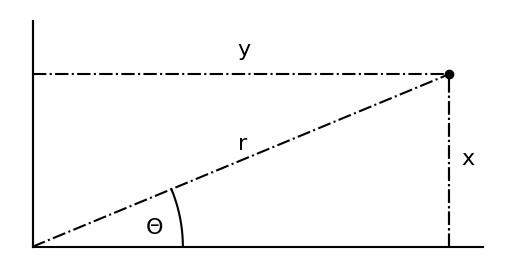
\includegraphics[width=6 cm]{wizualizacja.png}
\caption{Związek między biegunowym i kartezjańskim układem współrzędnych}
\end{center}
\end{figure}



Rozważmy teraz obrót wektora $\overrightarrow{v}$ o kąt $\psi$. Efektem obrotu jest powstanie wektora
$\overrightarrow{v}'=(r,\theta+\psi)$. Spróbujmy zapisać wektor $\overrightarrow{v}'$
przy użyciu współrzędnych kartezjańskich.

\begin{figure}[h]
\begin{center}
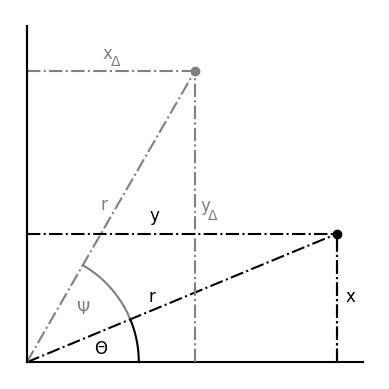
\includegraphics[width=6 cm]{wizualizacjaobrotu.png}
\caption{Wizualizacja obrotu punktu względem początku układu współrzędnych}
\end{center}
\end{figure}


$$x_\Delta=r\cos(\theta +\psi) =
r(\cos\theta \cos\psi - \sin \theta \sin \psi)=(r\cos\theta) \cos\psi -
(r\sin \theta) \sin \psi = x \cos\psi - y\sin \psi,$$
$$y_\Delta=r\sin(\theta +\psi)= r(\sin \theta \cos \psi +
\cos\theta \sin\psi) = (r\sin \theta) \cos \psi +
(r\cos\theta) \sin\psi  = x\sin\psi +y\cos\psi . $$

\subsection{Opis macierzowy obrotu}\label{SO(2)}
Powyższe równości możemy przedstawić za pomocą notacji macierzowej

$$
\begin{bmatrix}
x_\Delta\\
y_\Delta
\end{bmatrix} =
\begin{bmatrix}
\cos\psi   & -\sin\psi \\
\sin\psi & \cos\psi  
\end{bmatrix}
\begin{bmatrix}
x \\
y 
\end{bmatrix},
$$
Powyższą macierz kwadratową nazywamy macierzą obrotu na płaszczyźnie i oznaczamy jako
$\mathcal{R}_2(\psi)$.

\begin{defi}
Niech $A\in\mathcal{M}_n(\mathbb{R})$. Zbiór macierzy spełniający warunki:
\begin{enumerate}
	\item $ AA^t=I_n  A^tA,$
	\item $ det(A)=1,$
\end{enumerate}
nazywamy specjalną grupą ortogonalną przestrzeni $\mathbb{R}^n$ i oznaczamy ją jako 
SO($n$).
\end{defi}

Okazuję się każda macierz będąca elementem zbioru SO($n$), jest tak naprawdę opisem 
obrotu o pewien kąt w przestrzeni $\mathbb{R}^n$. Skupimy się teraz na dowodzie dla $n=2$,
w następnym rozdziale po przedstawieniu macierzy obrotu dla przestrzeni $R^3$, 
popełnimy dowód dla $n=3$.
\begin{twr}\label{rotationMatrixSO(2)}
Niech $A\in\textup{SO}(2)$. Wówczas $A$ jest macierzą obrotu na płaszczyźnie liczb rzeczywistych.
\end{twr}
\begin{dowod}
Niech $A=[a_{ij}]$ będzie dowolną macierzą ze zbioru SO($2$).
Oznacza to, że $A^t = A^{-1}$ oraz $\textup{det}A=\textup{det}A^t=\textup{det}A^{-1}=1$.
Z pierwszej równości dowiadujemy się, że macierz $A$ ma tak naprawdę postać
$$\begin{bmatrix}
a_{11}&-a_{12} \\
a_{12} & a_{11}
\end{bmatrix}.$$
Dodatkowo z drugiej równości wynika, że $\textup{det}A = a^2_{11}+a^2_{12}=1$.
W takim razie, posiłkując się wzorem na jedynkę trygonometryczną,
istnieje taki kąt $\psi$, że  $a_{11}=\cos\psi$ i $a_{12}=\sin\psi$.
Podsumowując, dowolna macierz ze zbioru SO($2$) jest tak naprawdę
opisem obrotu o pewien kąt na płaszczyźnie rzeczywistej.
\end{dowod}

\begin{prz}\label{exT_rotation}
W ramach przykładu dokonamy obrotu litery T, o kolejno $\frac{\pi}{2}$, $\pi$, $\frac{3\pi}{2}$.
Zacznijmy od narysowania litery. Zauważmy, że by narysować literę T, wystarczy w
odpowiedni sposób połączyć $8$ dokładnie dobranych punktów.
Punktami jakimi posłużymy się w wygenerowaniu litery T, są:
$$x_1 = (10,1),x_2 = (11,1),x_3 = (11,6),x_4 = (13,6),$$
$$x_5 = (13,7),x_6 = (8,7),x_7 = (8,6),x_8 = (10,6).$$
By wygenerować omawianą literę wystarczy w linii prostej połączyć punkt
$x_i$ z punktem $x_{i+1}$, gdzie $i\in\{1,2,...,8\}$. Dodatkowo,
łączymy punkt $x_8$ z $x_1$, uzyskujemy w ten sposób krzywe zamkniętą
w kształcie litery T.

\begin{figure}[h]
\begin{center}
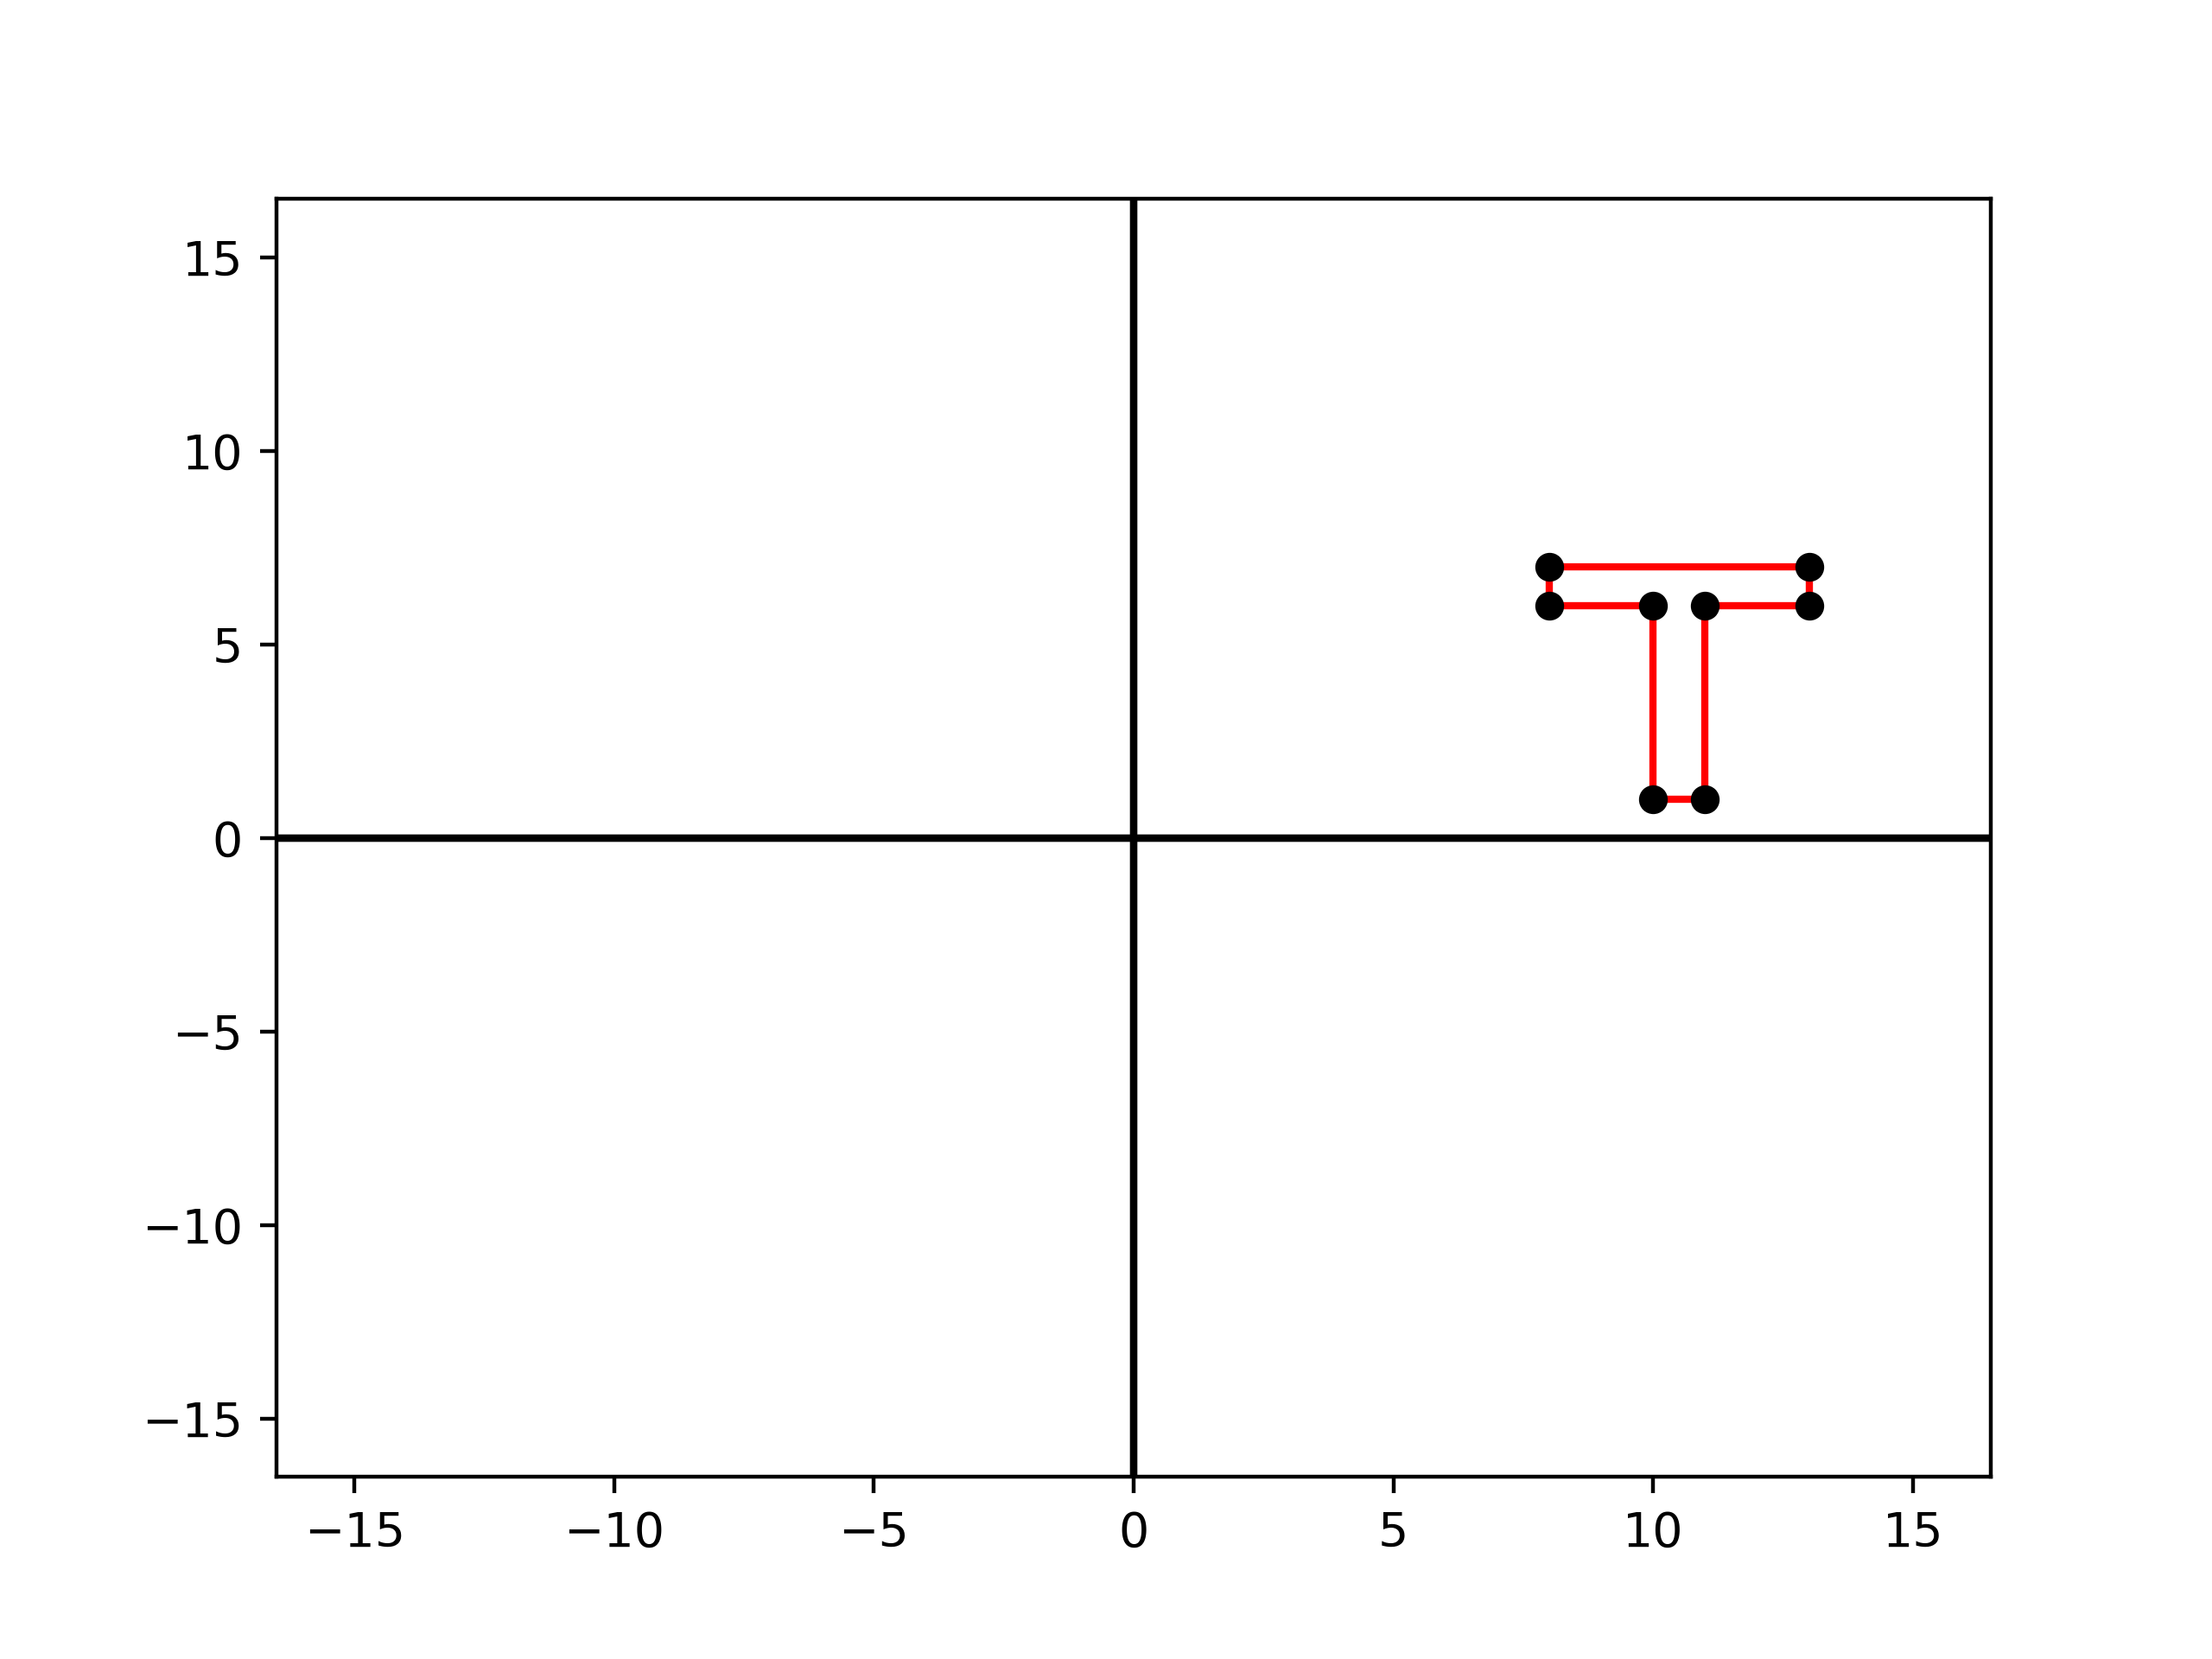
\includegraphics[width=7 cm]{T_samo.png}
\caption{Wygenerowana za pomocą powyższych instrukcji litera $T$.}
\end{center}
\end{figure}
\newpage

By obrócić literę $T$ wystarczy, że obrócimy punkty, które posłużyły do jej narysowania.
By to zrobić skorzystamy z macierzy obrotu dla  $\frac{\pi}{2}$, $\pi$, $\frac{3\pi}{2}$.
Mają one postać odpowiednio
$$R_\frac{\pi}{2}=\begin{bmatrix}
0&-1 \\
1&0 
\end{bmatrix},
R_\pi=\begin{bmatrix}
-1&0 \\
0&-1 
\end{bmatrix},
R_\frac{3\pi}{2}=\begin{bmatrix}
0&1 \\
-1&0 
\end{bmatrix}.
$$
W tym monecie wystarczy każdy z punktów przemnożyć przez powyższe macierze,a otrzymane wyniki będą 
obróconymi punktami. Punkty te łączymy w taki sam sposób, co oryginalne. W efekcie otrzymujemy:
\begin{figure}[h]
\begin{center}
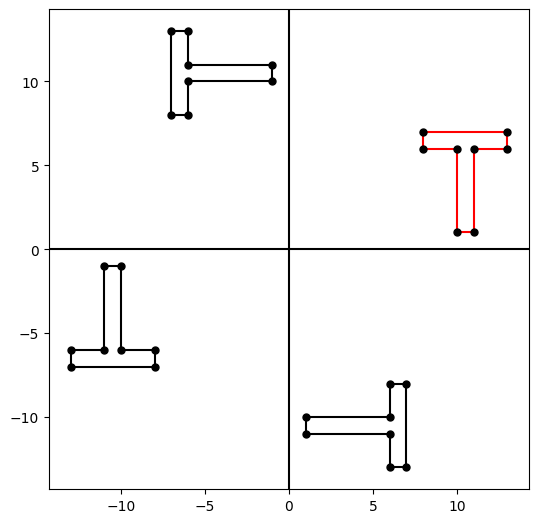
\includegraphics[width=7 cm]{T_obroty.png}
\caption{Kolorem czarnym zaznaczono litery $T$ obrócone o wcześniej podane macierze, kolorem szarym znaczono
obroty ,,przejściowe" w celu lepszej prezentacji zasady działania obrotu.}
\end{center}
\end{figure}
\end{prz}


\subsection{Macierze odbicia}
Naturalnym pytaniem po zapoznaniu się z macierzami obrotu, jest co w przypadku gdy macierz
ortogonalna posiada wyznacznik równy $-1$. W dowodzie do twierdzenie \ref{rotationMatrixSO(2)}.
udało nam pokazać, że dowolna macierz ortogonalna w $\mathcal{M}_2(\mathbb{R})$ jesteśmy 
w stanie zapisać w postaci
$$\begin{bmatrix}
\cos\theta&\sin\theta \\
\sin\theta & \cos\theta
\end{bmatrix}.$$
Pamiętając o tym jak wygląda macierz obrotu, możemy wywnioskować, że dowolną macierz 
ortogonalna stopnia $2$ o elementach rzeczywistych, której wyznacznik jest równy -$1$ ma postać
$$\begin{bmatrix}
\cos\theta&-\sin\theta \\
\sin\theta & -\cos\theta
\end{bmatrix}.$$

Rozważmy zatem ,,obrót" pewnego punktu $(x,y)\in\mathbb{R}^2$ o kąt równy $0$, jednak zamiast typowej macierzy obrotu użyjemy nam powyższej macierzy. W efekcie otrzymujemy 

$$\left\{\begin{array}{l}
x_\Delta = x \cos 0 - y\sin 0 =x\\
y_\Delta = x \sin 0 - y\cos 0 = -y
\end{array} \right. . $$

Efektem wykonanego ,,obrotu" jest odbicie lustrzane pierwotnego punktu względem osi $y$.
Pytaniem na jakie spróbujemy teraz odpowiedzieć to jak wygląda zmiana kąta wpływa na odbicie. 
By odpowiedzieć na to pytanie powtórzymy obrót litery $T$ z przykładu \ref{exT_rotation}.
\begin{prz}
W celu lepszej wizualizacji wykorzystamy te same punkty $x_1,...,x_8$ oraz połączymy je w taki sam sposób
jak w przykładzie  \ref{exT_rotation}. Dla ułatwienia zapisu wprowadźmy pewne oznaczenia. 
Oznaczmy, zatem
$$\mathcal{O}(\theta) =\begin{bmatrix}
\cos\theta_n&\sin\theta_n \\
\sin\theta_n & \cos\theta_n
\end{bmatrix}.$$
Katy ,,obrotu" dzięki, których użyjemy do określenia wartości elementów powyższej macierzy
będą elementami zbioru $\left\{\frac{2\pi x}{10}: x\in\mathbb{N}\cup\left\{ 0 \right\} \wedge x\leqslant10 \right\}$. Podane punkty przemnożymy przez zdefiniowane w ten sposób macierze.
Wynik wizualizujemy na płaszczyźnie w następujący sposób:
\begin{itemize}
\item[•] kolorem czerwonym zaznaczymy boki oryginalnej litery T,
\item[•] kolorem szarym zaznaczymy boki ,,obróconej" litery T.
\end{itemize}
W efekcie otrzymujemy  
\begin{figure}[h]
\begin{center}
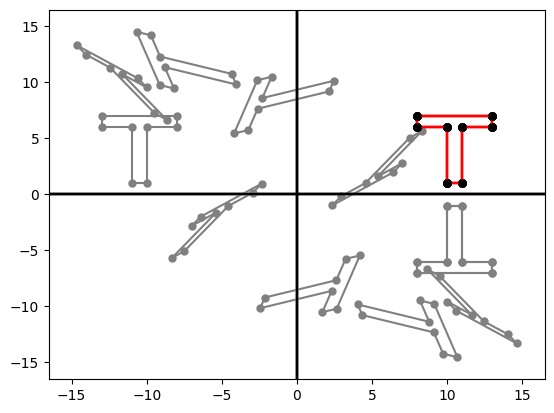
\includegraphics[width=7 cm]{T-reflection.png}
\caption{Wizualizacja odbicia}
\end{center}
\end{figure}
Możemy łatwo zauważyć, że dokonanie ,,obrotu" macierzami 
ortogonalnymi o wyznaczniku równym $-1$ nie spełnia założeń obrotu. Najbardziej widoczne
jest to na porównaniu pól obróconej litry T z jej pierwotną. W powyższym przykładzie tylko 
$2$ obroty mają identyczne pola co do wyjściowej. ,,Obroty" te zostały wykonane przez macierze
$$
\begin{bmatrix}
1&0 \\
0 & -1
\end{bmatrix},
\begin{bmatrix}
-1&0 \\
0 & 1
\end{bmatrix}.$$
Okazuje się, że przemnożenie dowolnego punktu przez dwie powyższe macierze daje w efekcie kolejno
odbicie względem osi $y$ oraz odbicie osi $x$.
\end{prz}
Z powyższego przykładu możemy wywnioskować, że mnożenie przez macierze ortogonalne 
o wyznaczniku równym $-1$ ma mało wspólnego z obrotem, za to dużo więcej z odbiciem. Z tego 
względu na zakończenie tej sekcji wprowadźmy dwie nowe definicje. 
\begin{defi}
Macierz ortogonalną stopnia $n$ o elementach rzeczywistych, której wyznacznik jest równy $-1$ 
nazywamy macierzą odbicia w przestrzeni $n$. 
\end{defi}
\begin{defi}
Zbiór składający się z macierzy ortogonalną stopnia $n$ o elementach rzeczywistych, nazywamy grupą
ortogonalną stopnia $n$. Omawiany zbiór oznaczamy jako $\textup{O}(n)$.
\end{defi}


\subsection{Opis obrotu za pomocą liczb zespolonych}
Alternatywnym sposobem opisu obrotu na płaszczyźnie $\mathbb{R}^2$
jest użycie liczby zespolonych. Wówczas dowolny punkt o współrzędnych kartezjańskich $(a,b)$
jesteśmy w stanie przedstawić w postaci $a+bi$, gdzie $a,b$ są liczbami rzeczywistymi, natomiast 
$i$ jest jednostką urojoną spełniającą warunek $i^2 = -1$. Powyższy sposób zapisu nazywamy 
postacią kanoniczną liczby zespolonej.\\
Alternatywnym sposobem zapisu $a+bi$ jest postać trygonometryczna. Przedstawia się ona w sposób
$|z|(\cos\theta+i\sin\theta),$
gdzie $\|z\| =\sqrt{a^2+b^2}$, $\theta=\textup{arctg}\frac{b}{a}$.\\

Rozważmy teraz mnożenie liczb zespolonych. Niech $z_1 = z_1(\cos\theta +i\sin\theta)$ oraz 
niech $z_2 = r_2(\cos\psi +i\sin\psi)$.
Wówczas mnożenie przedstawia się wzorem
$$z_1z_2=r_1r_2(\cos(\theta+\psi) +i\sin(\theta+\psi)).$$
Zauważmy, że by dokonać obrotu liczby zespolonej o kąt $\psi$ 
wystarczy pomnożyć ją przez liczbę postaci $$\cos\psi +i\sin\psi.$$
Korzystając z powszechnie znanego wzoru Eulera, obrót na płaszczyźnie
o kąt równy $\psi$ możemy interpretować jako pomnożenie przez $e^{i\psi}$.
Podsumowując, obrót punktu na płaszczyźnie możemy interpretować jako mnożenie liczb zespolonych.

\section{Obrót w przestrzeni w r3}

W tym rozdziale skupimy się na opisie obrotu w
przestrzeni $\mathbb{R}^3$. 
Począwszy od opisu macierzowego obrotu dookoła osi $x$, $y$ oraz $z$, następnie
rozważymy postać macierzy dookoła dowolnej osi obrotu.

\subsection{Kierunek obrotu}

W przestrzeni trójwymiarowej ważne jest ujednolicenie obrotu między osiami.
W tym celu kierunek obrotu będzie u nas wyznaczała powszechnie znana metoda
o nazwie ,,reguła prawej dłoni". W ramach przypomnienia działania reguły, jeśli ustawimy
kciuk prawej dłoni wzdłuż osi wokół której chcemy
dokonać obrotu, to zgięte palce będą przedstawiać kierunek obrotu.
Dzięki takiemu ujednoliceniu obrotu mamy tak naprawdę trzy osobne obroty względem osi $x,y$
oraz $z$.

\begin{figure}[h]
\begin{center}
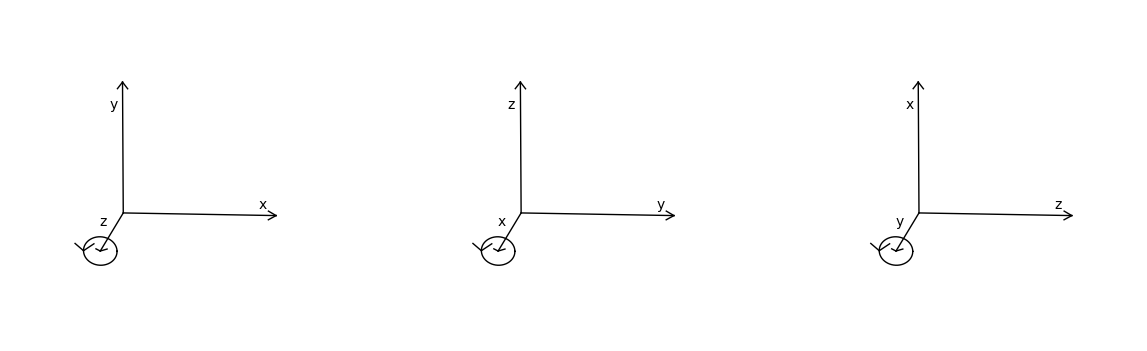
\includegraphics[width=15 cm]{zasPrawejReki.png}
\caption{Wizualizacja zasady prawej ręki w przestrzeni $\mathbb{R}^3$}
\end{center}
\end{figure}

\subsection{Opis macierzowy obrotu w przestrzeni}
W tym podrozdziale skupimy się na znalezieniu macierzy 
obrotu dla przestrzeni $\mathbb{R}^3$. W tym celu 
dla pewnego losowego punktu w tej przestrzeni dokonamy obroty względem głównych 
osi układu współrzędnych. 

Niech $p=(x_p,y_p,z_p)$ będzie pewnym punktem w $\mathbb{R}^3$. Zamodelujmy teraz
obrót punktu $p$ względem osi $z$, o kąt równy $\psi$. 
Dodatkowo niech $p_\Delta=(x_{p_\Delta},y_{p_\Delta},z_{p_\Delta})$ będzie punktem w $\mathbb{R}^3$, 
który jest efektem rozważanego obrotu. 
Zauważmy, że wartość współrzędnej
odpowiadająca osi $z$ nie ulega zmianie. Zmieniają się współrzędne odpowiadające osi $x$ oraz $y$.
W takim razie, możemy skorzystać ze wzorów wyprowadzonych z podrozdziału \ref{obrot2drozdzial}.
Podsumowując
$$\left\{\begin{array}{l}
x_{p_\Delta} = x_{p_\Delta} \cos\psi - y_{p_\Delta}\sin\psi \\
y_{p_\Delta}=x_{p_\Delta}\sin\psi + y_{p_\Delta}\cos\psi\\
z_{p_\Delta} = z_{p_\Delta}
\end{array}\right. \Longleftrightarrow \begin{bmatrix}
x_{p_\Delta}\\
y_{p_\Delta}\\
z_{p_\Delta}
\end{bmatrix} =
\begin{bmatrix}
\cos\psi   & -\sin\psi&0 \\
\sin\psi & \cos\psi & 0\\
0&0&1
\end{bmatrix}
\begin{bmatrix}
x_{p} \\
y_{p} \\
z_{p}
\end{bmatrix}.$$
Powyższa macierz kwadratowa jest macierzą obrotu względem osi $z$ o kąt równy $\psi$, oznaczać będziemy ją jako $\mathcal{R}_z(\psi)$.\\. 
W sposób analogiczny jesteśmy w stanie zdefiniować obrót względem pozostałych osi.\\
Macierz obrotu względem osi $x$ o kąt $\psi$ ma postać
 $$\begin{bmatrix}
 1&0&0\\
0&\cos\psi   & -\sin\psi\\
0&\sin\psi & \cos\psi
\end{bmatrix},$$
oznaczać będziemy ją jako $\mathcal{R}_x(\psi)$.\\
Natomiast, macierz obrotu względem osi $y$ o kąt $\psi$ ma postać
$$\begin{bmatrix}
\cos\psi&0&\sin\psi\\
0&1   & 0\\
-\sin\psi &0 & \cos\psi
\end{bmatrix},$$
oznaczać będziemy ją jako $\mathcal{R}_y(\psi)$.\\
W ten oto sposób udało nam się rozważyć obrót na trzech podstawowych osiach.

%obroe wokol roznych osi
\subsection{Wielokrotne obroty}
Pytaniem na jakie spróbujemy teraz odpowiedzieć będzie to, czy kolejność obrotu ma znaczenie. Okazuje się, że ma bardzo duże znaczenie. 
Istotność kolejności obrotu pokażemy w poniższym przykładzie.
\begin{prz}\label{PrzykladWielokrotnyObrot}
W przykładzie rozważymy obrót punktu $p=(1,1,1)$ wokół osi $x,z$ 
o kąt równy w obu przypadkach $\frac{\pi}{2}$.
Macierze obrotu mają wówczas postać
$$
\mathcal{R}_z\left(\frac{\pi}{2}
\right)=
 \begin{bmatrix}
0   & -1&0 \\
1 & 0 & 0\\
0&0&1
\end{bmatrix},\mathcal{R}_x\left(\frac{\pi}{2}
\right)=\begin{bmatrix}
 1&0&0\\
0&0   & -1\\
0&1 & 0
\end{bmatrix}.$$
Zacznijmy od rozważenia przypadku, gdzie najpierw dokonujemy obrót względem osi $x$.
$$\begin{bmatrix}
 1&0&0\\
0&0   & -1\\
0&1 & 0
\end{bmatrix}\begin{bmatrix}
 1\\
1\\
1 
\end{bmatrix} = \begin{bmatrix}
 1\\
-1\\
1 
\end{bmatrix}. $$
Po wykonaniu pierwszego obrotu uzyskaliśmy punkt o współrzędnych $(1,-1,1)$.
Wykonajmy obrót otrzymanego punktu względem osi $z$.
$$\begin{bmatrix}
0   & -1&0 \\
1 & 0 & 0\\
0&0&1
\end{bmatrix}\begin{bmatrix}
 1\\
-1\\
1 
\end{bmatrix} = \begin{bmatrix}
 1\\
1\\
1 
\end{bmatrix}.$$
Efektem obrócenia punktu $p$ najpierw względem osi $x$, a następnie względem osi $z$ o kąt równy $\frac{\pi}{2}$ w obu przypadkach, jest otrzymanie punktu wyjściowego.
Rozważmy teraz sytuacje, gdzie najpierw dokonujemy obrotu względem osi $z$.
$$\begin{bmatrix}
0   & -1&0 \\
1 & 0 & 0\\
0&0&1
\end{bmatrix}\begin{bmatrix}
 1\\
1\\
1 
\end{bmatrix} = \begin{bmatrix}
 -1\\
1\\
1 
\end{bmatrix}.$$
Efektem obrócenia względem osi $z$ jest otrzymanie punktu $(-1,1,1)$.
Wykonamy ostatni obrót względem osi $x$.
$$\begin{bmatrix}
 1&0&0\\
0&0   & -1\\
0&1 & 0
\end{bmatrix}\begin{bmatrix}
 -1\\
1\\
1 
\end{bmatrix} = \begin{bmatrix}
-1\\
-1\\
1 
\end{bmatrix}. $$
Efektem obrócenia punktu $p$ najpierw względem osi $z$, a następnie względem osi $x$ o kąt równy $\frac{\pi}{2}$ w obu przypadkach, jest punkt $(-1,-1,1)$. 
W ten sposób udało nam się pokazać, że kolejność obrotu względem osi ma znaczenie.
\end{prz}

Zauważmy, że dowolny obrót w przestrzeni $\mathbb{R}^3$ jesteśmy w stanie przedstawić
w postaci 
$(\psi,\theta,\gamma)$, gdzie 
\begin{itemize}
\item[$\bullet$] $\psi$ jest kątem obrotu względem osi $z$,
\item[$\bullet$] $\theta$ jest kątem obrotu względem osi $y$,
\item[$\bullet$] $\gamma$ jest kątem obrotu względem osi $x$.
\end{itemize}
Wyżej wymienioną trojkę nazywamy kątem Eulera.
\subsection{Macierz obrotu względem dowolnej osi obrotu}
Rozważmy teraz sytuację kiedy obracamy pewien punkt
najpierw o kąt równy $\phi$ względem osi $z$, następnie o kąt $\theta$ względem
osi $y$, kończąc na obrocie o kąt $\psi$ względem osi $x$.
Zacznijmy od pomnożenia obrotu względem osi $x$ przez obrót względem osi $y$.
$$
\mathcal{R}_y(\theta)\mathcal{R}_x(\psi)=\begin{bmatrix}
\cos\theta&0&\sin\theta\\
0&1   & 0\\
-\sin\theta &0 & \cos\theta
\end{bmatrix}
\begin{bmatrix}
 1&0&0\\
0&\cos\psi   & -\sin\psi\\
0&\sin\psi & \cos\psi
\end{bmatrix}=
\begin{bmatrix}
\cos\theta&\sin\theta\sin\psi&\sin\theta\cos\psi\\
0&\cos\psi   & -\sin\psi\\
-\sin\theta &\cos\theta\sin\psi & \cos\theta\cos\psi
\end{bmatrix}.
$$

$$
\mathcal{R}_z(\phi)(\mathcal{R}_y(\theta)\mathcal{R}_x(\psi)) = 
\begin{bmatrix}
0&\cos\phi   & -\sin\phi\\
0&\sin\phi & \cos\phi\\
0&0&1
\end{bmatrix}
\begin{bmatrix}
\cos\theta&\sin\theta\sin\psi&\sin\theta\cos\psi\\
0&\cos\psi   & -\sin\psi\\
-\sin\theta &\cos\theta\sin\psi & \cos\theta\cos\psi
\end{bmatrix}.
$$ 
Otrzymany produkt pomnóżmy teraz przez macierz obrotu względem osi $z$.
$$\mathcal{R}_{z(\phi)y(\theta)x(\psi)} = \mathcal{R}_z(\phi)\mathcal{R}_y(\theta)\mathcal{R}_x(\psi) = \begin{bmatrix}
\cos\phi\cos\theta& \cos\phi\sin\theta\sin\psi -& \cos\phi\sin\theta\cos\psi + \\
& \sin\phi \cos\psi &\sin\phi \sin\psi\\
&&\\
\sin\phi\cos\theta&\sin\phi\sin\theta\sin\psi+   & \sin\phi\sin\theta\cos\psi- \\
&\cos\phi\cos\psi&\cos\phi \sin\psi\\
&&\\
-\sin\theta &\cos\theta\sin\psi & \cos\theta\cos\psi
\end{bmatrix}.$$
W ten sposób udało nam się znaleźć macierz obrotu dla kąta Eulera równego $(\phi,\theta,\psi).$

Sprawdzimy teraz, czy macierz $\mathcal{R}_{z(\phi)y(\theta)x(\psi)}$ jest 
elementem specjalnej grupy ortogonalnej w $\mathbb{R}^3$.\\
Zacznijmy od obliczenia wyznacznika macierzy. Zauważmy, że stosując rozwinięcie Laplace'a
na macierzach obrotu względem osi $x,y$ oraz $x$ na kolejno $1,2$ i $3$ kolumnie, mamy tak naprawdę
do obliczenia minor, który jest macierzą obrotu na płaszczyźnie $\mathbb{R}^2$. Oznacza to, że każda 
z macierzy wyżej wspomnianych macierzy ma wyznacznik równy $1$. 
W takim razie, korzystając z twierdzenia Cauchy'ego w produkcie wyznacznika otrzymujemy: 
$$\det\left(\mathcal{R}_{z(\phi)y(\theta)x(\psi)}\right) = 
\det \left( \mathcal{R}_z(\phi)\mathcal{R}_y(\theta)\mathcal{R}_x(\psi)\right) = 
\det \left( \mathcal{R}_z(\phi)\right)\det\left(\mathcal{R}_y(\theta)\right)
\det\left(\mathcal{R}_x(\psi)\right)=1.$$
Zostało nam pokazać, że macierzą odwrotną do $\mathcal{R}_{z(\phi)y(\theta)x(\psi)}$
jest jej macierz transponowana. Zaczynimy od zauważenia, że macierzami odwrotnymi dla 
$\mathcal{R}_{x},\mathcal{R}_{y},\mathcal{R}_{z}$ są ich macierze transponowane.
W takim razie 
$$\mathcal{R}_{z(\phi)y(\theta)x(\psi)}\mathcal{R}^T_{z(\phi)y(\theta)x(\psi)} = 
\mathcal{R}_z(\phi)\mathcal{R}_y(\theta)\mathcal{R}_x(\psi)
\left(\mathcal{R}_z(\phi)\mathcal{R}_y(\theta)\mathcal{R}_x(\psi)\right)^T=$$
$$=\mathcal{R}_z(\phi)\mathcal{R}_y(\theta)\mathcal{R}_x(\psi)
\mathcal{R}^T_x(\psi)\mathcal{R}^T_y(\theta)\mathcal{R}^T_z(\phi) = I_n.$$
W ten sposób udało nam się pokazać, że  $\mathcal{R}_{z(\phi)y(\theta)x(\psi)} \in \textup{SO}(3).$


Przedstawimy teraz, że inkluzja zachodzi również w drugą stronę, tzn. że każda macierz 
z specjalnej grupy ortogonalnej jest tak naprawdę macierzą obrotu w przestrzeni $R^3$. 
W tym celu przedstawię dowód dwóch lematów, które ułatwią nam prace nad ostatecznym dowodem.
\begin{lem}\label{lematDolematuSO3}
Niech $A\in\mathcal{M}_n(\mathbb{R})$, gdzie $n$ jest liczną naturalną nieparzystą.
Wówczas macierz $A$ posiada przynajmniej jedną rzeczywistą wartość własną.
\end{lem}
\begin{dowod}
Wartości własne macierzy $A$, znajdziemy obliczając miejsca zerowe jej wielomianu charakterystycznego.
$$p_A(\lambda) = \det(\lambda I_n-A) = \lambda^n + a_1\lambda^{n-1}+...+a_n,$$
gdzie $a_1,a_2,...,a_n$ są rzeczywistymi współczynnikami wielomianu charakterystycznego macierzy $A$.
Obliczmy teraz granice jakie przyjmuje $p_A(\lambda)$ w $-\infty$ oraz $\infty$.
$$\lim\limits_{\lambda\rightarrow -\infty} p_A(\lambda) = -\infty,$$
$$\lim\limits_{\lambda\rightarrow \infty} p_A(\lambda) =  \infty.$$
Ze względu na to, że $p_A(\lambda)$ jest funkcją ciągłą 
to musi istnieć przynajmniej jedno rzeczywiste miejsce
zerowe wielomianu charakterystycznego macierzy $A$. 
Oznacza to, że macierz $A$ posiada przynajmniej jedną rzeczywistą wartość własną.
\end{dowod}
\begin{lem}\label{lematDolematuSO3_2}
Niech $A\in\textup{O}(n)$, gdzie $n$ jest liczną naturalną nieparzystą. Niech dodatkowo
$\lambda_0$ będzie rzeczywistą wartością własną macierzy A. Wówczas $\lambda_0 = \pm 1$.
\end{lem}
\begin{dowod}
Z lematu \ref{lematDolematuSO3}. wiemy, że macierz $A$ pewną ma przynajmniej jedna rzeczywistą wartość
własną $\lambda_0$. Oznacza to, że istnieje odpadający wartości własnej $\lambda_0$, wektor własny
$v=[x_1,...,x_n]\in\mathbb{R}^n$ tzn. $Av=\lambda_0 v$. 
Pamiętając, że $A$ jest macierzą ortogonalną, przejdźmy wyprowadzenia pierwszej równości.
$$\lambda_0v^Tv = (\lambda_0 v)^T\lambda_0 v=(Av)^T Av = v^T A^T Av = v^T v .$$
W konsekwencji
$$\lambda_0^2v^Tv = v^T v\Rightarrow\lambda_0^2 = 1\Rightarrow \lambda_0 = \pm 1.$$
\end{dowod}
\begin{twr}
Jeśli $R\in\textup{SO}(3)$, to jest ona macierzą obrotu o pewien kąt.
\end{twr}
\begin{dowod}
Dzięki lematowi \ref{lematDolematuSO3_2}. wiemy, że rzeczywistą wartością 
własną macierzy $A$ jest $-1$ lub $1$. By pokazać prawdziwość powyższego twierdzenia
pokażemy jego prawdziwość najpierw z założeniem, że $1$ jest wartością własną macierzy $A$, a następnie
powtórzymy to dla wartości własnej równe $-1$.

Załóżmy zatem, że $1$ jest wartością własną macierzy $A$. Przypiszmy zatem do podanej wartości własnej
odpowiadający jej jednostkowy wektor własny $v_3\in \mathbb{R}$. Weźmy dodatkowo wektory $v_1,v_2$,
które będą bazą ortonormalną podprzestrzeni 
$v^\perp = \left\{ v\in\mathbb{R}^3 : v\circ v_3 = 0 \right\}$. Używając wektorów $v_1,v_2,v_3$ 
skonstruujmy macierz $B = [v_1,v_2,v_3]$, gdzie podane wektory są kolumnami macierzy. Zauważmy, że 
macierz $B$ jest macierzą ortogonalną. By to potwierdzić pomnóżmy macierz $B$ przez jej macierz transponowaną. 
$$
BB^T = [v_1,v_2,v_3]\left[\begin{array}{c}
v_1^T\\
v_2^T\\
v_3^T
\end{array}  \right],
$$
gdzie $v_1^T,v_2^T,v_3^T$ są wersami macierzy transponowanej $B$. Ze względu na to, że każdy z wektorów
jest prosto padły do pozostałych, to zachodzi równość 
$$v_i\circ v_j = 0,$$
gdzie $i,j\in \{1,2,3 \}$ przy czym $i\neq j $. Natomiast, w przypadku $i = j$ to powyższy iloczyn skarany
wynosi $1$, wynika to z faktu ortonormalności wektorów rozważanych wektorów. Podsumowując 
$$
BB^T = [v_1,v_2,v_3]\left[\begin{array}{c}
v_1^T\\
v_2^T\\
v_3^T
\end{array}  \right] = I_3,
$$
zatem udało nam się potwierdzić ortogonalność macierzy $B$. Oznacza to, że wyznacznik macierzy $A$
jest równy $1$ lub $-1$. Ze względu na to, że zamiana kolejności wierszy zmienia znak wyznacznika
wybierzemy wyznacznik równy $1$ bez straty ogólności.
Oznacz to, że $B\in\textup{SO}(3)$. W takim razie 
$$AB = [Bv_1,Bv_2,Bv_3],$$
pamiętając jednak o tym, że $v_3$ jest wektorem własnym macierzy $A$, zatem $Av_3 = v_3$.
Dodatkowo, iloczyn dwóch macierzy ortogonalnych również jest macierzą ortogonalną. Oznacza to, 
że macierz $AB$ jest macierzą ortogonalną. Dodatkowo, $Bv_1,Bv_2\in v_3^\perp$.
W takim razie $A(v_1)=av_1+bv_2$, $A(v_2)=cv_1+dv_2$, $A(v_3) = v_3$, co w konsekwencji daje nam macierz
$$B^{-1}AB\begin{bmatrix}
a&c   & 0\\
b&d & 0\\
0&0&1
\end{bmatrix}\in \textup{SO}(3) \Longrightarrow
\begin{bmatrix}
a&c\\
b&d 
\end{bmatrix}\in \textup{SO}(2).$$
Oznacza to, że macierz $A$ jest macierzą obrotu o pewien kąt.\\

Przypuśćmy teraz, że wartość własną macierzy $A$ jest równa $-1$. Niech $v_3$ będzie odpowiadającym
ortogonalnym wektorem własnym do podanej wartości własnej. Definiując macierz macierz $B$ w analogiczny
sposób jak wyżej otrzymujemy 
  $$B^{-1}AB\begin{bmatrix}
a&c   & 0\\
b&d & 0\\
0&0&-1
\end{bmatrix}\Longrightarrow \det\left(\begin{bmatrix}
a&c \\
b&d 
\end{bmatrix} \right) =-1.$$
Oznacza to, że $\begin{bmatrix}
a&c \\
b&d 
\end{bmatrix}$ jest elementem zbioru $\textup{O}(2)$. Oznacza to, że istnieje niezerowy wektor 
$v\in v^\perp_3$ taki, że $Av=v$. Oznacza  to, że $1$ jest również wartością własną macierz $A$.
W ten sposób udało nam się pokazać, że jeśli $A\in\textup{SO}(3)$ to jest ona tak naprawdę macierzą
obrotu.  
\end{dowod}
\subsection{Opis kwaternionowy obrotu w przestrzeni }
\begin{defi}
Kwaternion którego moduł jest równy $0$, nazywamy kwaternionem jednostkowym.
\end{defi}
\begin{defi}
Kwaternion którego część skalarna jest równa $0$, nazywamy czysto wektorową.
\end{defi}
\begin{wni}
Dowolny element z przestrzeni $\mathbb{R}^3$ jest możemy przedstawić w
postaci kwaternionu czysto wektorowego.
\end{wni}
\begin{twr}
Niech $q$ będzie kwaternionem jednostkowym w postaci $q=c+su$, gdzie $|u| = 1$, $c=cos\theta$
oraz $s=sin\theta$ dla $\theta\in[0,\pi]$. Wówczas odwzorowanie 
$T_q : \mathbb{R}^3\rightarrow \mathbb{R}^3$ zdefiniowane wzorem $T_q(v) = qvq^{-1}$ 
obraca punkt $v$ względem osi $u$ 
o kąt równy  $2\theta$ w kierunku przeciwnym do ruchu wskazówek zegara.
\end{twr}
\chapter{Zastosowanie}
\section{Implementacja obrotu w języku Python}
\subsection{Kwaterniony- Python}
W celu zaimplementowania obrotu przy użyciu kwaternionów, musimy zaimplementować
podstawowe działania algebraiczne na ciele kwaternionów do języka Python.
Zacznijmy od ustalenia jakiej postaci będziemy używać. Mianowicie postacią
kwaternionu jaką wykorzystamy jest postać Hamiltonowska $q=q_0+\overrightarrow{q}$.
Przy pomocy tej postaci zdefiniujemy funkcje, które umożliwią nam wykonanie 
działania $qvq^{-1}$.
 

Ze względu na postać hamiltonowską kwaternionu możemy skorzystać ze wcześniej podanego
wzoru mnożenia dla tej postaci. Jednak by zdefiniować mnożenie, będziemy musieli
zdefiniować $4$ nowe funkcje, których połączenie pomoże nam napisać
funkcje mnożenia. Przejdźmy do wypisania wszystkich potrzebnych funkcji i do
opisania ich działania.
\begin{itemize}
\item[$\bullet$] $dotProduct()$,
\item[$\bullet$] $crossProduct()$,
\item[$\bullet$] $scalarVector()$,
\item[$\bullet$] $addingVectorPart()$.
\end{itemize} 
W tym miejscu dobrze wspomnieć o założeniach jakie przyjąłem, 
w ramach pisania powyższych funkcji jak i pozostałych związanych z obrotem kwaternionów.
W ramach przyśpieszenia działania funkcji zdecydowałem się na niekorzystaniu z pętli czy
innych instrukcji warunkowych. Użycie funkcji warunkowych zwiększyło czas wykonywania 
obrotu przy pomocy kwaternionów niemal trzykrotnie.\\
Zacznijmy od opisania funkcji $dotProduct()$. Przyjmuje dwa argumenty typu ,,lista" rozmiaru $3$.
Reprezentują one część wektorową kwaternionów. Mnożymy odpowiadające sobie elementy list przez siebie, 
a następnie je dodajemy. Wynik powyższego działania zostaje zwrócony.
Funkcja $crossProduct()$ również przyjmuje dwa argumenty typu ,,lista" rozmiaru $3$.
Zadaniem jej jest obliczenie iloczynu wektorowego podanych dla podanych wartości.
Zwraca ona listę rozmiaru $3$. Funkcja $scalarVector()$ przyjmuje dwa argumenty
w odróżnieniu jednak od wyżej opisanych, pierwszym argumentem jest zmienna typu ,,float", drugą
natomiast jest lista rozmiaru $3$. Zadaniem funkcji jest przemnożenie wektora, przez podaną stała.
Zwraca ona listę o trzech trzech elementach. Ostatnia funkcja o nazwie $addingVectorPart()$ przyjmuje 
dwa argumenty typu ,,lista" rozmiaru $3$. Dodaje ona odpowiadające elementy do siebie
i zwraca listę o rozmiaru $3$.\\

Przy użyciu powyższych funkcji możemy zdefiniować funkcje $multiQuaternion()$, która posłuży 
do obliczenia iloczynu kwaternionów. Przyjmuje ona cztery argumenty, kolejno 
\begin{itemize}
\item[$\bullet$] $a_1$ zmienną typu ,,float",
\item[$\bullet$] $v_1$ zmienna typu ,,list" rozmiaru $3$,
\item[$\bullet$] $a_2$ zmienną typu ,,float",
\item[$\bullet$] $v_2$ zmienna typu ,,list" rozmiaru $3$.
\end{itemize} 
Zmienne $a_1$,$a_2$ traktujemy jako część skalarną kwaternionów, odpowiednio $v_1$ oraz $v_2$ interpretujemy
jako część wektorową. Funkcja zwraca listę o dwóch elementach, pierwszym z nich będzie
zmienna typu ,,float" rozumiana jako 
cześć skalarna nowo powstałego kwaternionu, natomiast drugim elementem będzie lista o trzech elementach,
którą interpretujemy jako część wektorową iloczynu.
Rozważmy teraz budowę powyższej funkcji. Pierwszy element który zwracamy jest tak naprawdę efektem
wynikiem działania $a_1-a_2 - dotProduct(v_1,v_2)$. Drugi element określamy przy użyciu funkcji
$crossProduct()$, $scalarVector()$ oraz $addingVectorPart()$.
Program zaczyna od obliczenia $crossProduct(v_1,v_2)$, $scalarVector(a_1,v_2)$ oraz $scalarVector(a_2,v_1)$.
Wyniki powyższych obliczeń są następnie sumowane za pomocą $addingVectorPart()$ oraz zwracane jako drugi
element listy. W ten oto sposób udało nam się skonstruować funkcje $multiQuaternion()$
obliczającą iloczyn kwaternionów.

By napisać funkcje dokonującą obrotu przy użyciu kwaternionów, potrzebujemy jeszcze napisać funkcje obliczając
sprzężenie. Funkcja $conjugateQuaternion()$ przyjmuje dwie zmienne jedną typu ,,float", drugą typu ,,list"
o długości trzech elementów. Zmienne odpowiadają odpowiednio części skalarnej oraz wektorowej kwaternionu.
Sposób działania funkcji polega na zmianie znaków elementom listy. $conjugateQuaternion()$ zwraca
listę złożoną z dwóch elementów, gdzie pierwszym z nich jest nie zmieniona pierwsza zmienna przyjęta 
przez funkcje, drugim natomiast jest przyjęta lista, której elementy mają zmieniony znak. W ten sposób
udało nam się przedstawić sprzężenie.

W ten sposób mamy już wszystkie składowe potrzebne do napisania funkcji $rotation_quaterion()$ mamy już gotowe.
Funkcja ta będzie przyjmowała trzy zmienne
\begin{itemize}
\item[$\bullet$] $angle$ zmienną typu ,,float",
\item[$\bullet$] $rotation_axis$ zmienna typu ,,list" rozmiaru $3$,
\item[$\bullet$] $element$ zmienna typu ,,list" rozmiaru $3$.
\end{itemize}  
Zmienna $angle$ jest kątem obrotu, $rotation_axis$ wektor określający oś obrotu, 
z kolei $element$ jest punktem przestrzeni $\mathbb{R}^3$ który chcemy
obrócić. Wewnątrz definicji funkcji zaczynamy od przekształcenia zmiennych $angle$ i 
$rotation_axis$ na kwaternion tym razem postaci trygonometrycznej.
Następnie obliczamy kwaternion odwrotny do podanego w zmiennych przy pomocy $conjugateQuaternion()$. Kolejno
przy pomocy $multiQuaternion()$ w odpowiedni dokonujemy mnożenia podanych 
podanych kwaternionów, przez co w efekcie otrzymujemy obrócony $element$, który jest zwracany w przez funkcje.
Opisana powyżej definicja funkcji jest najszybsza i zostanie ona użyta w benchmarku w kolejnym rozdziale,
jednak posiada ona pewną wadę. Podany przez nas $rotation_axis$ musi być kwaternionem o długości równej $1$.
Dlatego zdefiniujemy dodatkową funkcje obliczającą obrót, która będzie dokonywała normalizacji wektora
odpowiadającego osi obrotu.
W tym celu napiszemy funkcje $NormalizeVector()$, która jako argument będzie przyjmowała wektor
w formie listy o trzech elementach. Policzy od normę euklidesową dla tego wektora, a następnie
każdy z elementów zostanie przez nią podzielony. Nowo postały w ten sposób wektor zostanie przez tą funkcje zwrócony.
Ta prosta funkcja nie wpływa w dużym stopniu na czas wykonywania operacji, jednak w 
jeśli chcemy uzyskiwać jak najszybszy efekt, to powinniśmy z niej zrezygnować.
W rozdziale Wydajność zostanie przeprowadzony test dla obrotu z normalizacją jak i bez normalizacji.
\subsection{Macierzowy model obrotu}
Do przygotowania macierzowego modelu obrotu w języku Python skorzystamy z pakietu \textit{numpy}. 
Jedną z funkcji jaką zawiera ten pakiet jest $matmul()$, który umożliwia mnożenie macierzy. 
W celu zaprogramowania obrotu zdefiniowałem pięć nowych funkcji, o nazwach
\begin{itemize}
\item[$\bullet$] $xaxisMatrixrotation()$,
\item[$\bullet$] $yaxisMatrixrotation()$,
\item[$\bullet$] $zaxisMatrixrotation()$,
\item[$\bullet$] $rotationMatrixZYX()$,
\item[$\bullet$] $matrixRotation()$.
\end{itemize} 
Omówmy teraz sposób działania powyższych funkcji. Funkcje $xaxisMatrixrotation()$,\\
$yaxisMatrixrotation()$,
$zaxisMatrixrotation()$ jako przyjmują jeden argument typu $float$, a zwracają one macierz obrotu o kącie równym
argumentowi odpowiednio wokół osi $x,y$ oraz $z$. Są to funkcje bazowe, wywołujemy je w wewnątrz definicji
$rotationMatrixZYX()$, gdzie za pomocą funkcji $matmul()$ dokonujemy ich mnożenia. Funkcja ta przyjmuje trzy argumenty
typu $float$ oznaczmy je jako $\psi,\phi,\theta$, zwraca natomiast macierz obrotu względem kąta eulera $(\psi,\phi,\theta)$.
Ostatnia funkcja $MatrixRotation()$, przyjmuje dwa argumenty, pierwszym z nich jest macierz, natomiast drugim argumentem 
punkt. Macierz wykorzystuje $matmul()$ do przemnożenia argumentów miedzy sobą, a wynik tego mnożenia jest zwracany.

Założenia algorytmu obrotu są proste, $rotationMatrixZYX()$ wykorzystuje funkcje\\
$xaxisMatrixrotation()$, $yaxisMatrixrotation()$, $zaxisMatrixrotation()$ do obliczenia 
macierzy obrotu dla podanego przez nas kąta eulera. Wygenerowana w ten sposób macierz służy jako argument
dla funkcji $MatrixRotation()$, która dokonuje na drugim argumencie dokonuje obrotu co jest zwracane przez nią.

Mamy zatem zdefiniowane mnożenie, pozostaje jeszcze zdefiniować funkcje 
\subsection{Kwaternionowy model obrotu}
\section{Wydajność}
W celu porównania ze sobą metody obu metod obrotu wykonamy test, dzięki któremu porównamy ich wydajność ze sobą. Zacznijmy od nadania testowi pewnego kontekstu.

Horizont: Zero Down, jest grą która miała swoją premierę w na początku $2017$. Gra ta zasłynęła głównie ze względu na aspekty 
techniczne gry, takie jak otwarty świat, czy co 
dla nas ciekawsze jakości wykonanych modeli graficznych. Jedną z informacji jaką podzieli się twórcy gry
są detale dotyczące modelu głównej bohaterki gry o imieniu Aloy. Otóż model głównej bohaterki składał się 
z około $550$ tyś. trójkątów sklejonymi ze sobą zwanych potocznie ,,poligonami". 
Dla uproszczenia załóżmy, że model Aloy, możemy przedstawić za pomocą dokładnie $550$ tyś punktów.
W ramach określenia wydajności modeli dokonamy obroty pewnego zbioru punktów o mocy równej $550$ tyś, co
będzie reprezentować model głównej bohaterki gry Horizont: Zero Down.  
\subsection{Kontrukcja benchmark'u}
Test będzie składał się z dwóch niezależnych od segmentów, jednakże w każdym z nich będziemy obracać 
ten sam zbiór punktów. Zanim przejdziemy do opisania poszczególnych segmentów, omówię 
generowanie zbioru punktów.
Zbiór punktów reprezentujący 'Aloy' zostanie utworzony przy pomocy pakietu 
\textit{random} do języka Python, a będąc precyzyjnym skorzystamy z funkcji o nazwie \textit{random}(),
która zwraca losowy punkt w przedziału $[0,1]$. 
Zbiór ten będzie generować pętla, która będzie powtarzać się $550$ tyś. razy i w każdym cyklu do 
listy będzie dodawać trójelementową listę złożą z elementów pochodzących z funkcji \textit{random}.
W celu uproszczenia zapisu w dalszej części oznaczmy powyższy zbiór punktów jako $\mathcal{A}$.
\subsection*{Test wydajności względem jednej osi obrotu}
Pierwszy test jaki wykonamy będzie testem, w którym model 'Aloy' będziemy obracać o stały kąt względem jednej osi. Zasymilujemy w ten sposób obrót nieruchomego modelu, często prezentowanego podczas
procesu produkcji. Sposób jaki wykonamy test wygląda następująco, za pomocą funkcji \textit{linspace} 
z biblioteki \textit{numpy} wygenerujemy listę o długości $300$. Lista ta będzie zawierała kąt obrotu 
względem osi z. Przyjmujemy długość równą $300$, by założony obrót postaci trwał $10$ sekund, gdzie na
jedną sekundę przypada $30$ klatek obrazu. W celu określenia wydajności zmierzymy czas, jaki zajęłoby
wygenerowanie obrotu przy użyciu metody macierzowej oraz kwaternionowej. Dodatkowo by uzyskać większa
wiarygodność wyników test powtórzymy $10$ razy by wyciągnąć średnią z czasów dla obu metod.
By zachować czytelność czas trwania danego testu zaokrąglamy do sekund.\\

Wyniki z wyżej opisanego testu przedstawia poniższa tabela:
\begin{table}[h]
\begin{tabular}{|c|c|c|c|c|c|c|c|c|c|c|c|}
\hline
      Numer testu &  $1.$  &  $2.$  &  $3.$  &  $4.$ &  $5.$ &  $6.$ &  $7.$ &  $8.$ &  $9.$ &  $10.$ & Średnia \\ \hline
Model Kwat. &$402$&$414$&$428$&$437$&$438$&$445$&$450$&$432$&$442$&$461$& $434.9$      \\ \hline
Model Macierzowy    &$415$&$430$&$427$&$427$&$383$&$354$&$360$&$355$&$346$&$354$& $385.2$       \\ \hline
\end{tabular}
\end{table}
\subsection*{Test wydajności względnej zmiennej osi obrotu}
Drugi test obejmuje założenie, że każdy punkt ma inną oś obrotu. 
Sytuacja ta występuje np. w przypadku, gdy postać porusza się. 
W tym celu musimy delikatnie zmienić kod benchmarku. Siła obrotu przy użyciu macierzy było to, że na
jedną generowaną klatkę obrazu wystarczyło wygenerować jedną macierz obrotu, co jest powolnym procesem.
W tym przypadku, dla każdego punktu musimy wygenerować osobną macierz obrotu podczas generowania jednej klatki.
Problem podobnej natury nie występuje w przypadku obrotu metodą obrotu związaną z kwaternionami.\\

Test wykonamy w następujący sposób. Tak jak wcześniej dokonamy obrotu każdego punkty ze zbioru $\mathcal{A}$ i jak wcześniej
każdy z punktów obrócimy $300$ razy. Różnica polega na tym, że w przypadku obrotu macierzowego będziemy obracać o kąt Eulera
równemu obracanemu elementowi. Natomiast w przypadku obrotu modelem kwaternion, kątem obrotu będzie wartość uzyskana wcześniej
z wcześniej wspomnianej funkcji \textit{random}(), jednakże każdy z punktów będzie posiadał inną oś obrotu. Będąc dokładnym
dla $x=(x_{1},x_{2},x_{3})\in\mathcal{A}$ osią obrotu będzie wektor definiowany wzorem 
$\frac{1}{r}[x_{1},x_{2},x_{3}]$, gdzie $r$ jest odległością w rozumieniu Euklidesa punktu $x$ od środka układu współrzędnych.
Łatwo zauważyć, że oba obroty nie są identyczne, nie powinno to jednak wpłynąć na wiarygodność testu.\\

Wyniki z wyżej opisanego testu przedstawia poniższa tabela:

\begin{table}[h]
\begin{tabular}{|c|c|c|c|c|c|c|c|c|c|c|c|}
\hline
 Nr testu   & $1.$&$2.$ &  $3.$  &  $4.$ &  $5.$ &  $6.$ &  $7.$ &  $8.$ &  $9.$ &  $10.$ & Średnia \\ \hline
Kwat.      &$457$&$458$&$440$&$439$&$439$&$439$&$437$&$437$&$450$&$449$&  $444.5$   \\ \hline
Macie. &$1767$&$1769$&$1768$&$1768$&$1768$&$1759$&$1757$&$1757$&$1759$&$1765$& $1763.7$       \\ \hline
\end{tabular}
\end{table}

\subsection*{Wniosek}
Pierwszym wnioskiem jaki nasuwa się po po wykonaniu testów jest to, że wybór macierzowego 
modelu obrotu ma sens w momencie, gdy możemy sobie pozwolić na generowaniu małej liczby
macierzy obrotu podczas tworzenia pojedynczej klatki obrazu. Na podstawie testu pierwszego 
powinniśmy wykonać obrót szybciej o około $11.5\%$. 
W momencie kiedy mamy do czynienia z sytuacją, kiedy chcemy obrócić każdy punkt o inny kąt, 
zdecydowanie lepszym wyborem jest kwaternionowy model obrotu. Dzięki testowi drugiemu
udało nam się pokazać, że obrót z użyciem kwaternionu jest prawie $3$-krotnie szybszy od
alternatywnego modelu obrotu macierzowego. Dodatkowo można zauważyć, że średnia czasu obrotu metodą kwaternionów 
z testu $1$ oraz $2$ rożni się od siebie o prawie $10$ sekund. Wynika to z faktu, użycia normalizacji co spowolniło proces.\\

Z powyższego testu wynika, że zdecydowanie bardziej użyteczna jest metoda obrotu przy użyciu kwaternionów. 
Obrót macierzowy jest szybszy, ale pojedynczych przypadkach. W ogólności metoda kwaternionowa jest zdecydowanie szybsza.
Najbardziej optymalne, oczywiście byłoby połączenie ty dwóch metod obrotu. Należy jednak pamiętać, że samo połączenie 
ich ze sobą może spowolnić proces co może spowodować nieopłacalność syntezy algorytmów.   
\section{Konstrukcja bączka}
W tym rozdziale skupimy się na opisaniu konstrukcji bączka, którego obrót będziemy symulować w dalszej części pracy.
Zauważmy, że bączkiem możemy nazwać stożki sklejone ze sobą podstawami. 
W punkcie $(0,0,0)$ będzie znajdowała się podstawa, punkt styku bączka
z podłożem, którym w naszym przypadku jest płaszczyzna $z=0$. Punk ten będzie wierzchołkiem naszego pierwszego bączka,
jego podstawą będą elementy należące do zbioru \\
$\lbrace (x,y,z)\in\mathbb{R}^3: x^2+y^2 = 1, z=1\rbrace$. Zbiór ten oznaczmy jako $P_1$. W ten sposób udało nam się uzyskać prowizoryczny bączek, dodajmy jednak ze względów estetycznych drugi stożek. Wierzchołkiem drugiego stożka ustawimy w punkcie
$(0,0,3)$, natomiast jego podstawą będzie zbiór 
$\left\lbrace (x,y,z)\in\mathbb{R}^3: x^2+y^2 = \left(\frac{1}{3}\right)^3, z=\frac{11}{10}\right\rbrace$. Oznaczmy go jako
$P_2$. W ten sposób otrzymujemy dwa stożki, które po połączaniu ze sobą podstaw z opowiadającymi sobie punktami utworzą 
bączek.\\

By narysować stożek za pomocą powyższego modelu będziemy musieli określić precyzje rysunku. Wynika to z faktu nieprzeliczalności
zbiorów $P_1$ oraz $P_2$. Oznacza to, że im więcej punktów wybierzemy tym bardziej model bączka będzie dokładniejszy.
Pamiętajmy jednak o tym, że zwiększenie dokładności modelu spowoduje zwiększenie czasu trwania generowania obrazu.
Zacznijmy od narysowania szkieletu oraz głównych punktów bączka przy użyciu $10$ elementów ze zbiorów $P_1$ oraz $P_2$.
\begin{figure}[h]
\begin{center}
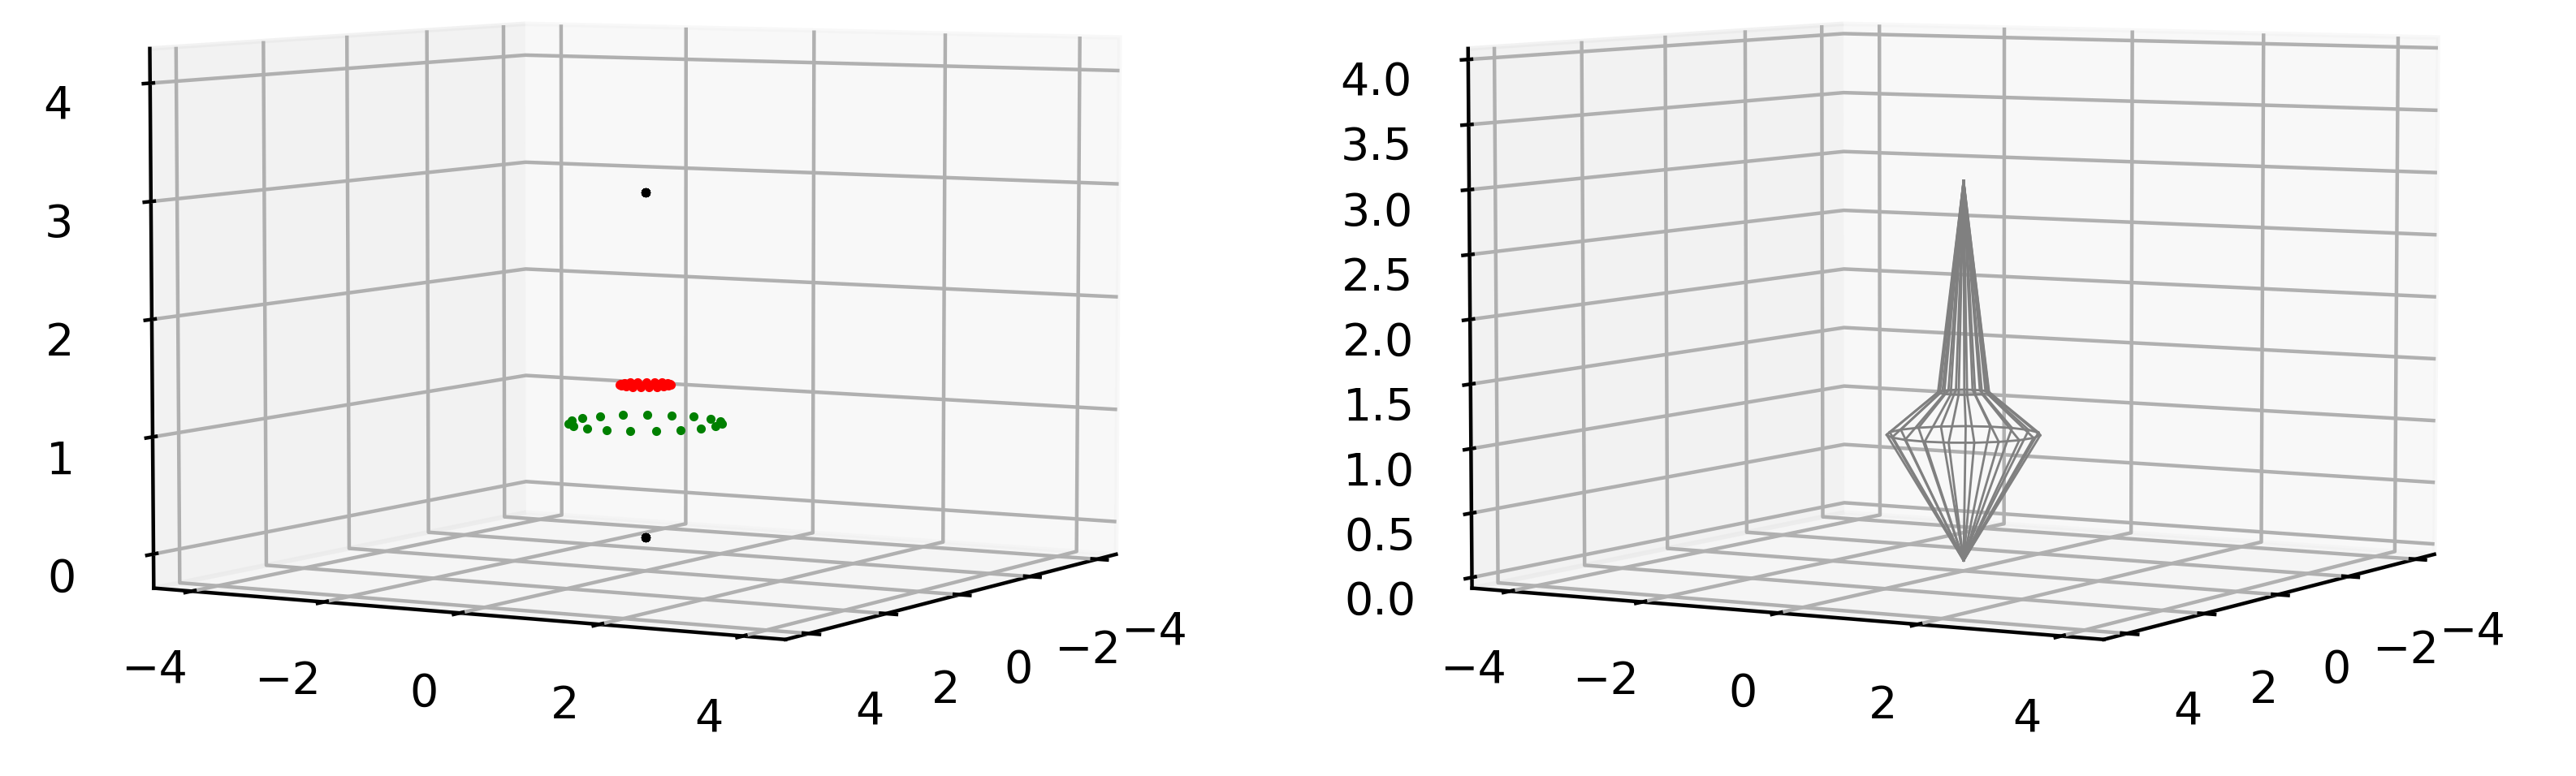
\includegraphics[width=12 cm]{skrech.png}
\end{center}
\end{figure}

Na obrazku po lewej stronie widzimy punkty, których połączenie w odpowiedni sposób skutkuje powstaniem modelu bączka 
(rysunek prawy). Kolorem zielonym zaznaczone zostały elementy zbioru $P_1$, natomiast czerwonym elementy zbioru $P_2$.
Na rysunku prawym przedstawiony został szkic modelu bączka przy pomocy punktów bazowych. W tym miejscu warto zauważyć,
że powyższy szkic tak naprawdę składa się z trójkątów oraz czworokątów sklejonych ze sobą brzegami. 
Łatwo obliczyć, że powyższy model składa się z $30$ wielokątów. 

Wyżej wykonane rysunki mają jednak pewną wadę konstrukcyjną, w celu ich narysowania wykorzystaliśmy funkcje 
\textit{plot3d} z pakietu $matplotlib$. Świetnie sprawuje się ona do rysowania wykresów, czy prostych szkiców, jednak
sensowne zaprezentowanie obrotu za jej pomocą nie jest możliwe. W tym celu skorzystamy z funkcji $Poly3DCollection()$,
z tego samego pakietu, jako wartości przyjmuje ona punkty, które są zamieniane na wielokąty, 
których kolor możemy ustawić. Ustawienie różnych kolorów w naszym przypadku jest niezwykle ważnie,
ponieważ ustawienie bączka jednokolorowego lub ustawienie takiego samego koloru dla poszczególnej warstwy spowoduje
,że obrót bączka nie będzie zauważalny. Przejdźmy zatem do narysowania modelu bączka, którego ruch będziemy w dalszej
części pracy modelować: 
\begin{figure}[h]
\begin{center}
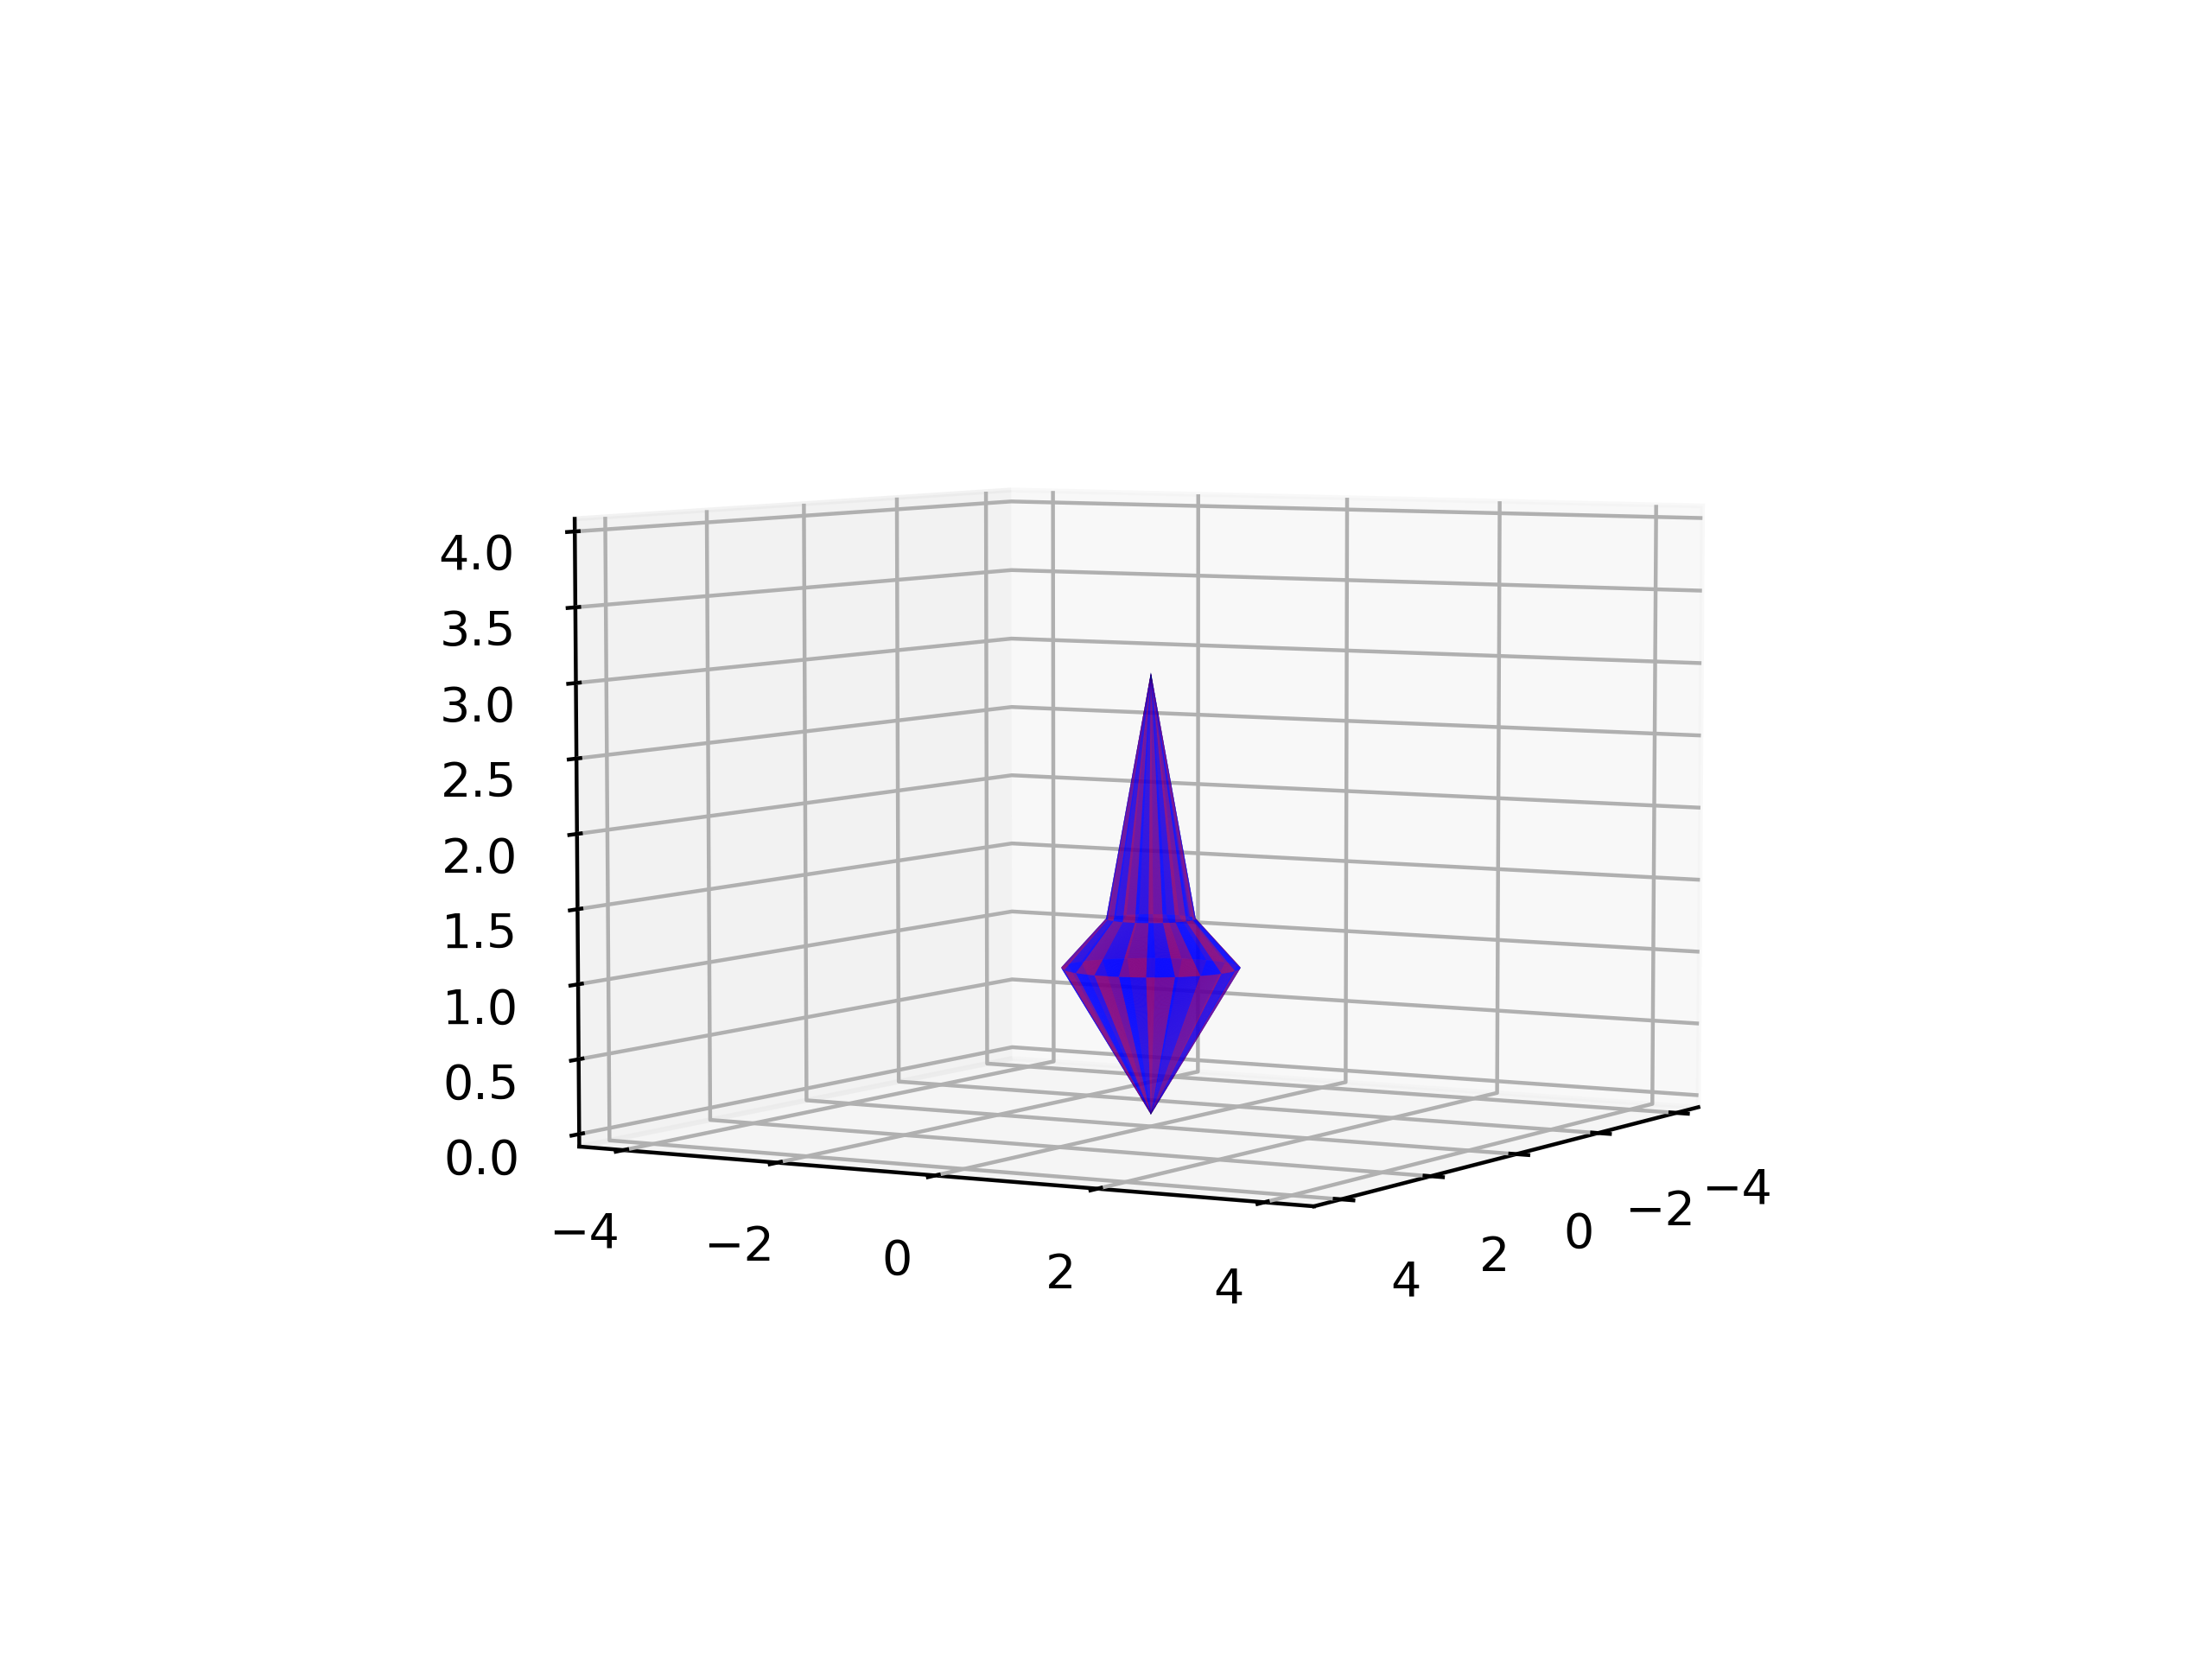
\includegraphics[width=10 cm]{top_0.png}
\end{center}
\end{figure}

By dokonać obrotu powyższej figury musimy tak naprawdę obrócić punkty, które są używane do utworzenia wielokątów.
W ramach prezentacji zasady działania dokonamy obrotu powyższego bączka, względem dwóch osi o pewne kąty. 
Pierwszą z nich będzie oś $z$, o drugą oś obrotu dokładnie opiszemy w dalszej cześć pracy w części
gdzie będziemy modelować ostateczny model bączka.

\begin{figure}[h]
\begin{center}
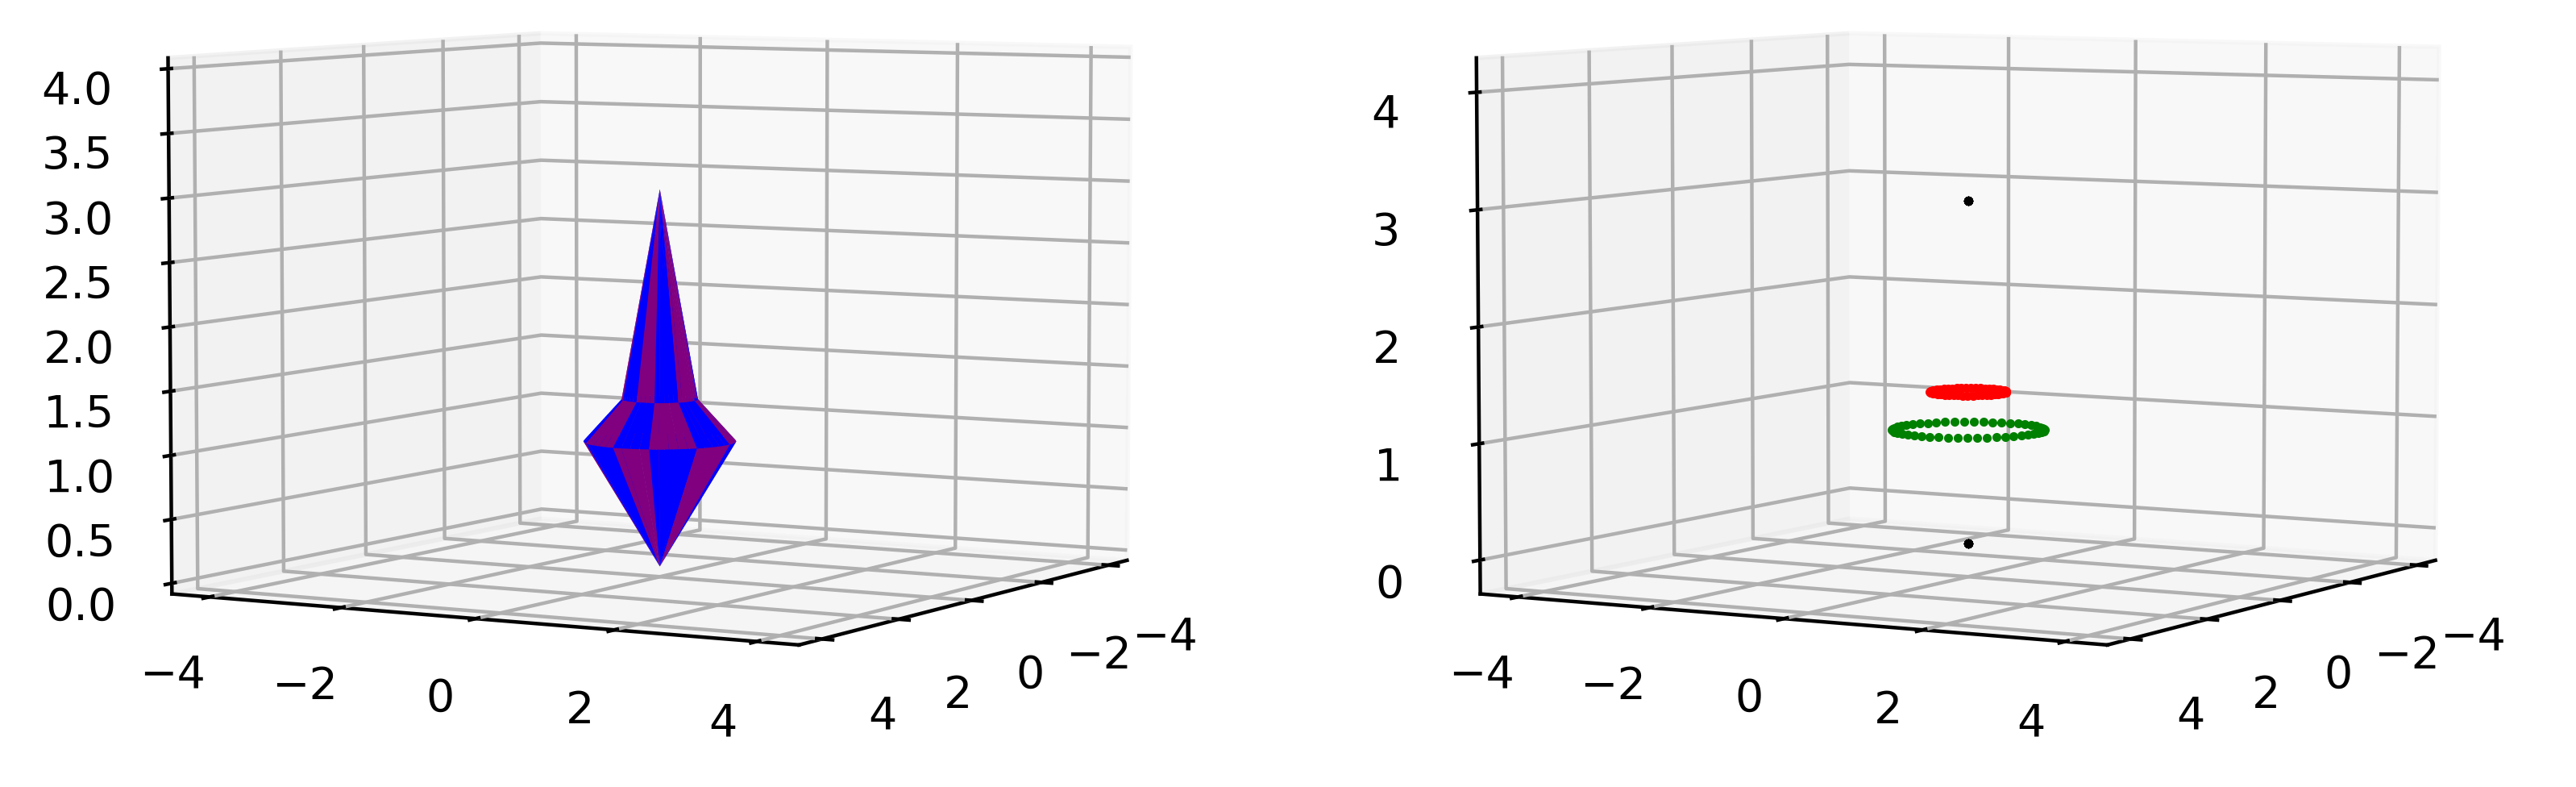
\includegraphics[width=10 cm]{0.png}
\end{center}
\end{figure}
\newpage
\begin{figure}[h]
\begin{center}
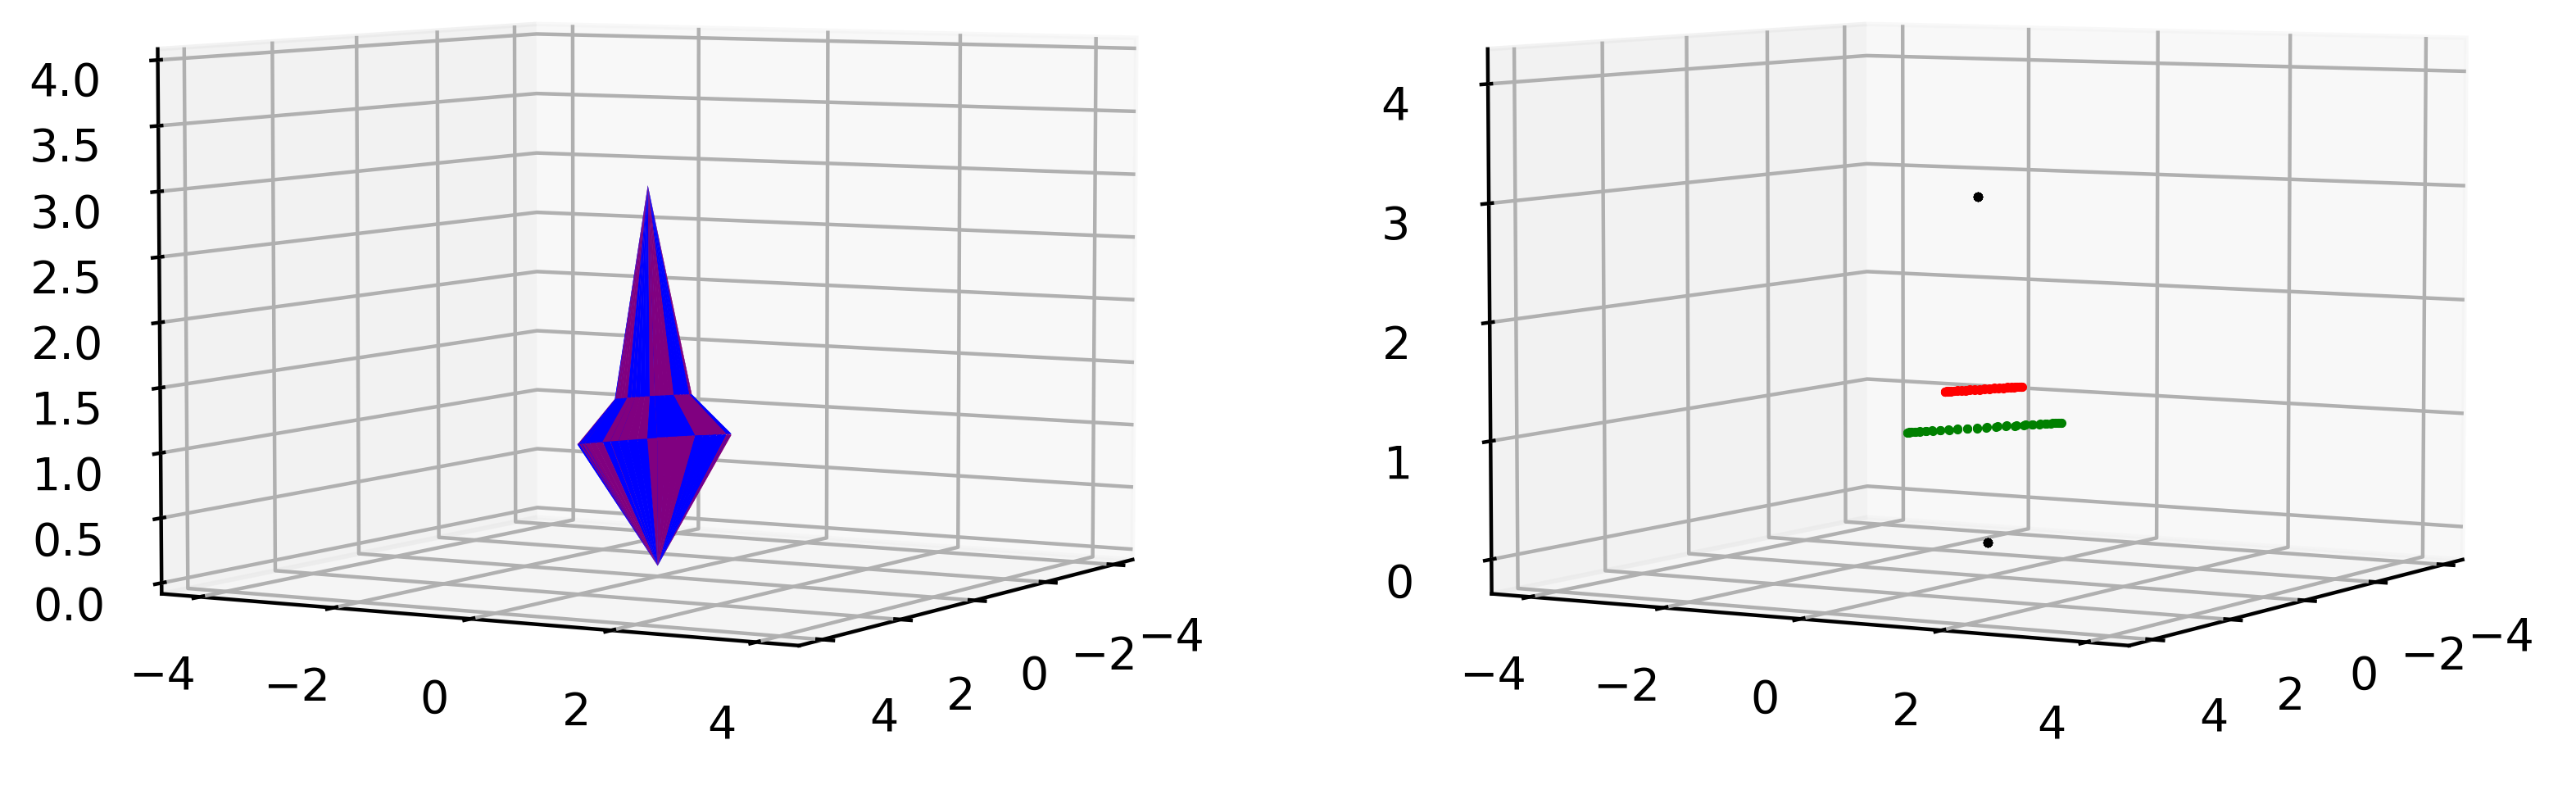
\includegraphics[width=10 cm]{1.png}
\end{center}
\end{figure}
\begin{figure}[h]
\begin{center}
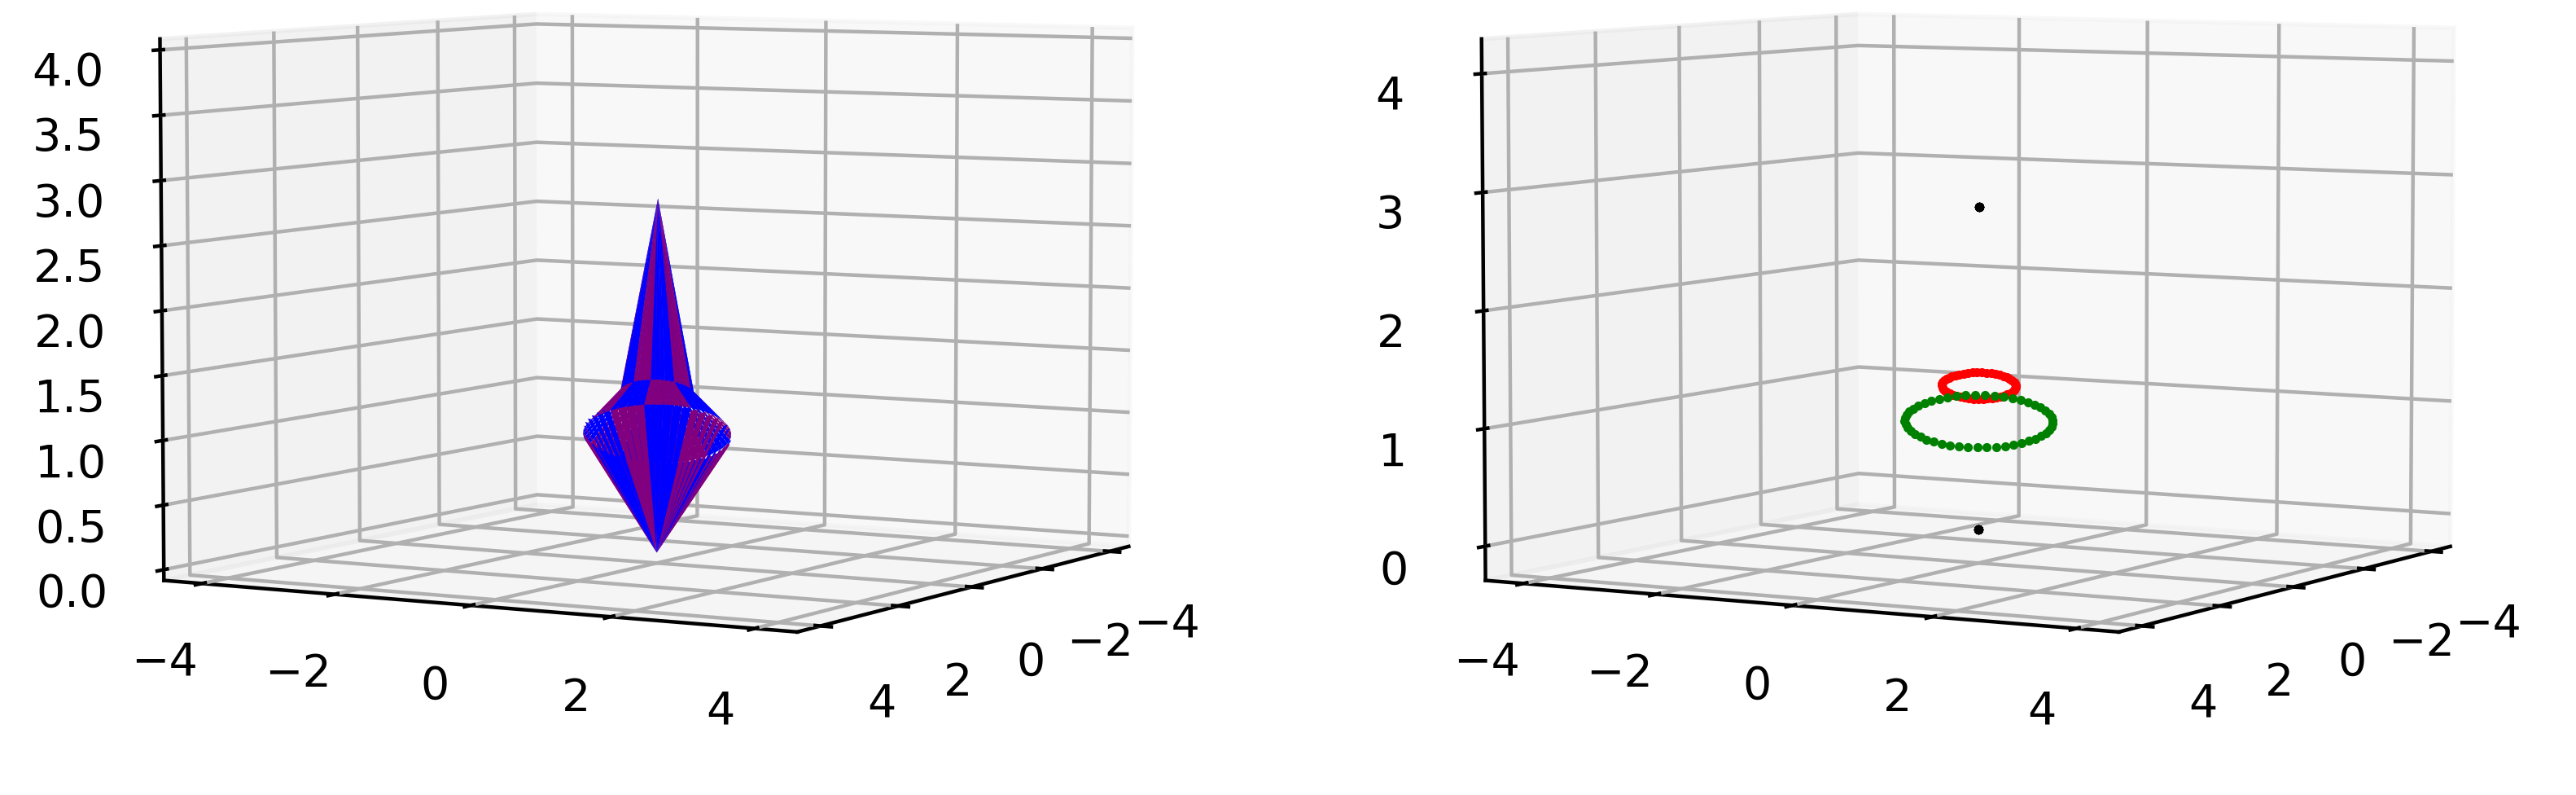
\includegraphics[width=10 cm]{2.png}
\end{center}
\end{figure}
Powyższe rysunki przedstawią, że by dokonać obrotu bączka wystarczy obrócić 
punkty, które służą do utworzenia wielokątów. Warto w tym miejscu zauważyć,
że punkt $(0,0,0)$ nie zależnie od wykonanego na nim obrotu, nie zmieni się.

Ostateczny model bączka, będzie składał się z łącznie $1000$ elementów ze zbiorów $P_1$ oraz $P_2$ oraz wierzchołków naszych stożków, co w sumie daje $2002$ punktów. Oznacza to, że model naszego bączka będzie składał się z $6$ tyś. wielokątów.
\section{Ostateczny model i przygotowywanie animacji}
Rozdział zaczniemy od skonstruowania wcześniej wspomnianego modelu bączka składającego się $6$ tyś. wielokątów.
Następnie napiszemy funkcje, która będzie obracać bączek metodą macierzową, jak i przy użyciu kwaternionów.

Konstrukcje bączka nie zmienia się w porównaniu do wcześniej wygenerowanych modeli. 
Główną różnicą w porównaniu do wcześniejszych modeli jest liczba elementów wyciąganych ze zbiorów
$P_1$ oraz $P_2$. Zacznijmy od opisania procesu wyciągania elementów.

Przy użyciu funkcji $linspace()$ z pakietu $numpy$. Funkcja ta wyciąga przyjmuje $7$
zmiennych, jednak nam wystarczy skorzystać z $3$, pozostałe $4$ są opcjonalne i nie ma potrzeby ich podawania.
Pierwszym argumentem jaki przyjmuje jest zmienna $start$, w naszym przypadku oznaczać ona będzie początek przedziału. Drugim elementem jaki przyjmuje jest zmienna $stop$, odpowiednio do wcześniejszego 
oznacza koniec przedziału. Ostatnią zmienną jest $num$, która służy do określenia liczby próbek do wygenerowania.
Funkcja ta, w formie listy zwraca $num$ równo odległych punktów z przedziału $[start,stop]$.
W naszym przypadku zwraca nam listę zawierającą $1000$ równo odległych punktów z przedziału $[0,2\pi]$.
Przy użyciu powyższej listy możemy wygenerować dwie nowe listy, których elementy należą odpowiednio do 
zbioru $P_1$ oraz $P_2$. Punkt odpowiadający za wierzchołek oraz punkt odpowiadający
za czubek stożka podajemy manualnie. W ten sposób uzyskaliśmy wszystkie główne punkty, które możemy użyć do
wygenerowania wielokątów przy użyciu $Poly3DCollection()$, które sklejone będą utworzą stożek.
W celu ustawieniu różnych kolorów wielokątów skorzystamy z instrukcji warunkowej $if$ oraz z ustawionej przez
nas stałej o nazwie $color\_change\_frequency$ typu $int$. Kolory na jakie się zdecydowałem to, żółty oraz
czarny.     
\begin{figure}[h]
\begin{center}
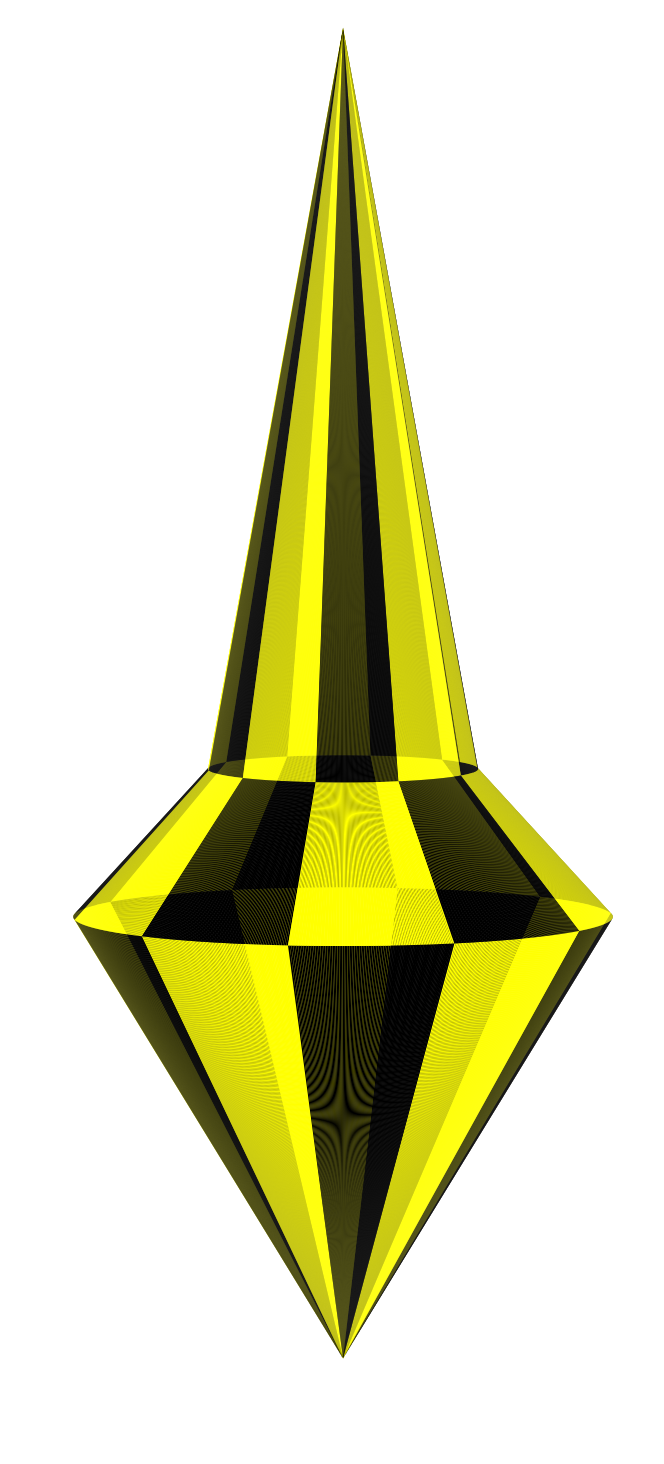
\includegraphics[width=3 cm]{test0.png}
\caption{Ostateczny model bączka składającego się z $6$ tyś. wielokątów.}
\end{center}
\end{figure} 
W taki sposób udało nam się wygenerować model bączka, przejdźmy teraz do konstrukcji obrotu w celu wykonania animacji rotacji bączka.
\subsection{Animacja w przy użyciu obrotu kwaternionowego}
Mamy wygenerowane punkty, pozostaje je teraz odpowiednio obrócić. W tym podrozdziale przygotujemy funkcje,
która posłuży do rotacji rozważanego stożka oraz omówimy model rotacji.

Ruch bączka możemy przyrównać do precesji. Ruch ten oznacza zmiany kierunku obrotu osi obracającego ciała. 
Oś obrotu obraca się wówczas pewnego kierunku zakreślając w ten sposób powierzchnie boczą bączka. Jednakże,
w naszym przypadku oś obrotu będzie zakreślała z czasem coraz większe koło. Wynika to z faktu utraty, 
że bączek z czasem traci prędkość obrotu co kończy się jego upadkiem. Zacznijmy od za modelowania 
obrotu bączka, bez uwzględniania jego upadania.

Łatwo zauważyć, że prędkość obrotu bączka możemy określić za pomocą obrotu względem osi $z$. Im większą prędkość obrotową chcemy uzyskać tym większy kąt obrotu musimy podać. Problematyczne wydaje się za modelowanie stopniowe
opadanie bączka. Zacznijmy od za modelowania ruchu bączka nachylonego bączka, który się nie obraca wokół własnej osi. Rozważmy osie, którą wyznaczają wektory $[r\cos(x_i),r\sin(x_i),\sqrt{1-r^2}]$, gdzie
$r = \frac{1}{2}$, $x_i=\frac{\pi}{2}i$ oraz $i\in\{1,2,3,4\}$. Dokonamy obrotu względem powyższych osi 
o kąt równy stały kąt, równy $\frac{\pi}{2}$. Efektem obrotu jest ruch precesyjny, co dobrze przedstawia 
poniższa grafika.
\begin{figure}[h]
\begin{center}
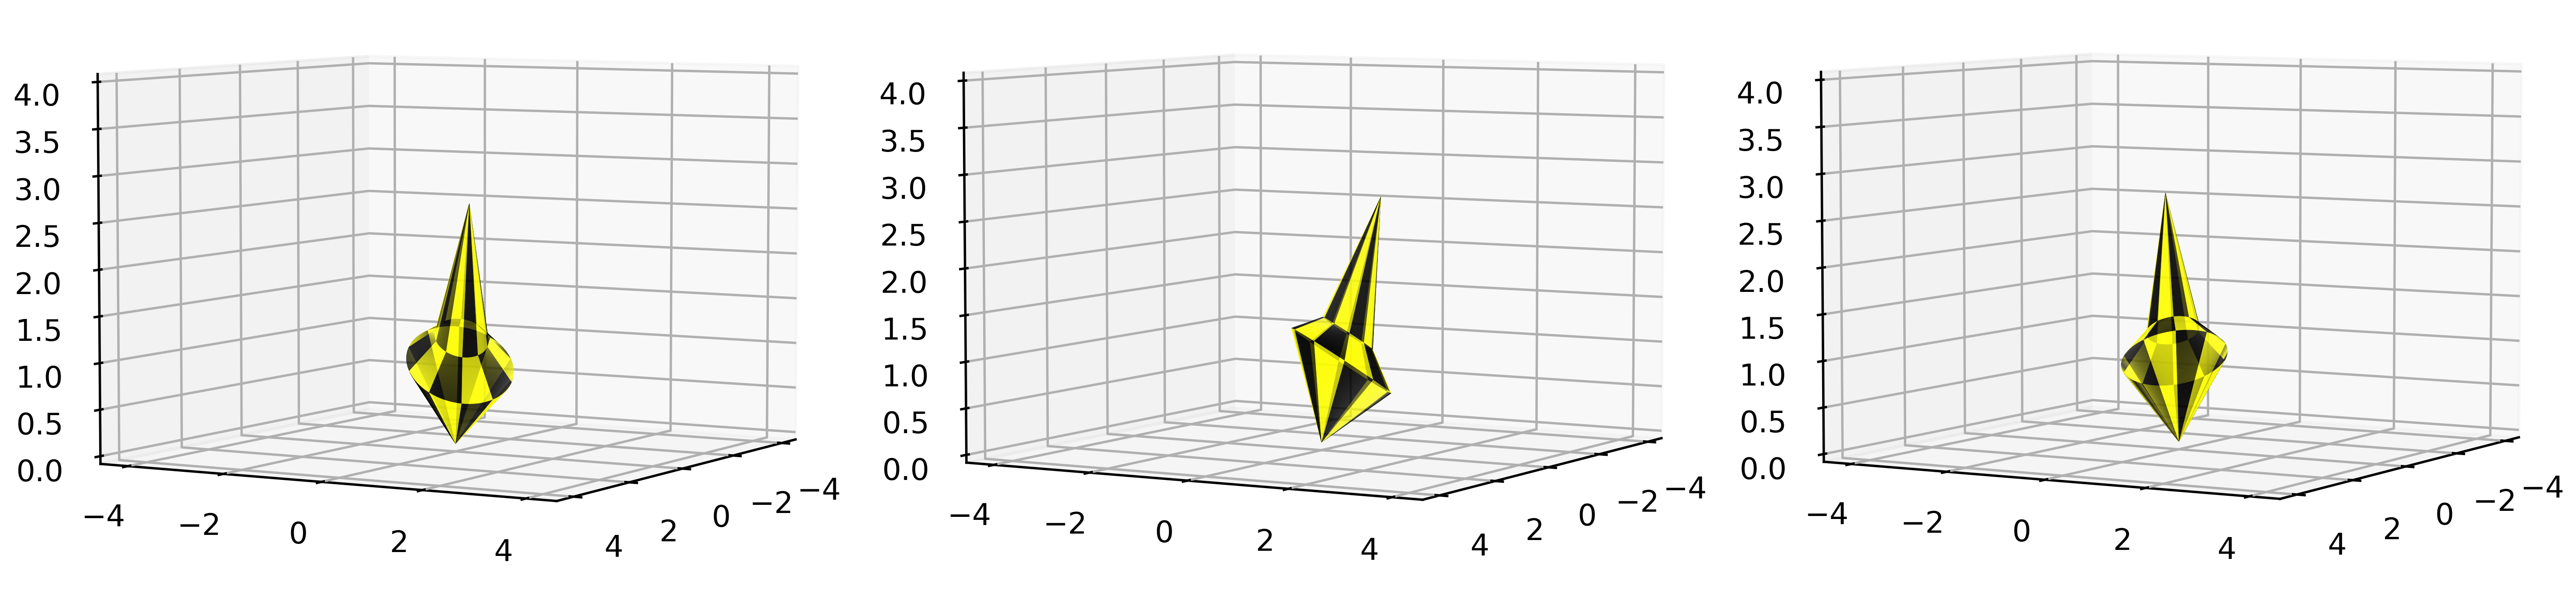
\includegraphics[width=15 cm]{precesja.png}
\caption{Wizualizacja obrotu względem osi określonej przez $\left[r\cos(x_i),r\sin(x_i),\sqrt{1-r^2}\right]$, o kąt
 $\frac{\pi}{2}$}
\end{center}
\end{figure}
By za modelować stopniowe opadanie bączka wartość $r$ w wektorze określającym oś, wraz z czasem z $0$
powinna stopniowo się zwiększać. Połączenie dwóch wyżej opisanych obrotów, posłuży nam za ostateczne za modelowanie ruchu bączka.

Funkcja jaka posłuży nam do obrotu bączka to $spin3d()$. Przyjmuje ona 4 zmienne,
\begin{itemize}
\item[$\bullet$] $speed$ zmienną typu ,,float",
\item[$\bullet$] $angle$ zmienną typu ,,float",
\item[$\bullet$] $axis\_rotation$ zmienna typu ,,list" rozmiaru $3$,
\item[$\bullet$] $time$ zmienna typu ,,int".
\end{itemize}
Zmienne $speed$ oraz $angle$ odpowiadają za kąt obrotu odpowiednio względem osi $z$ i osi określanej przez $axis\_rotation$. Zmienna $time$ wpływa jedynie na nazwę pliku, będziemy jej używać do odpowiedniego 
połączenia obrazków w celu uzyskania animacji. Wygenerujemy teraz $500$ obrazków, a następnie przy pomocy
pakietu $imageio$ połączymy obrazki, będą one zmieniały się co $20$ milisekund. Oznacza to, że nasz animacja
będzie trwała $10$ sekund oraz, że w nasza animacja będzie w $50$ klatach na sekundę.
Ustalmy teraz jakie wartości przyjmie funkcja dla każdej klatki.
Zbiory z jakich będziemy wyciągać wartości przedstawiają się w następujący sposób:
\begin{itemize}
\item[$\bullet$] $axisAngle = [0,32\pi]$,
\item[$\bullet$] $radius = \left[0,\frac{1}{4}\right]$,
\item[$\bullet$] $speedValue = $ .
\end{itemize}
Z każdego zbioru wyciągamy po $500$ równo odległych elementów i wykorzystamy do tego wcześniej używaną funkcje 
$linspace()$. Wartość ze zbioru $speedValue$ użyjemy jako zmiennej $speed$, do zmiennej 
$axis\_rotation$ wprowadzamy listę postaci 
$[r\cos(angle),r\sin(angle),\sqrt{1-r}]$, gdzie $r$ jest elementem ze zbioru $radius$, a $angle$ należy do
zbioru $axisAngle$. Do generowania obrazów wykorzystamy pętle $while$, z warunkiem $time < 500$.
Zmienna $time$ na początku przyjmie wartość $0$, jednak podczas działania pętli będziemy do niej dodawać $1$
za każde przejście cyklu. Zmienne $time$ wykorzystamy również jako ostatni parametr w zdefiniowanej funkcji o
tej samej nazwie.
Poniżej zamieszczam $10$ klatek obrazu, które wchodzą w skład animacji.
\begin{figure}[h]
\begin{center}
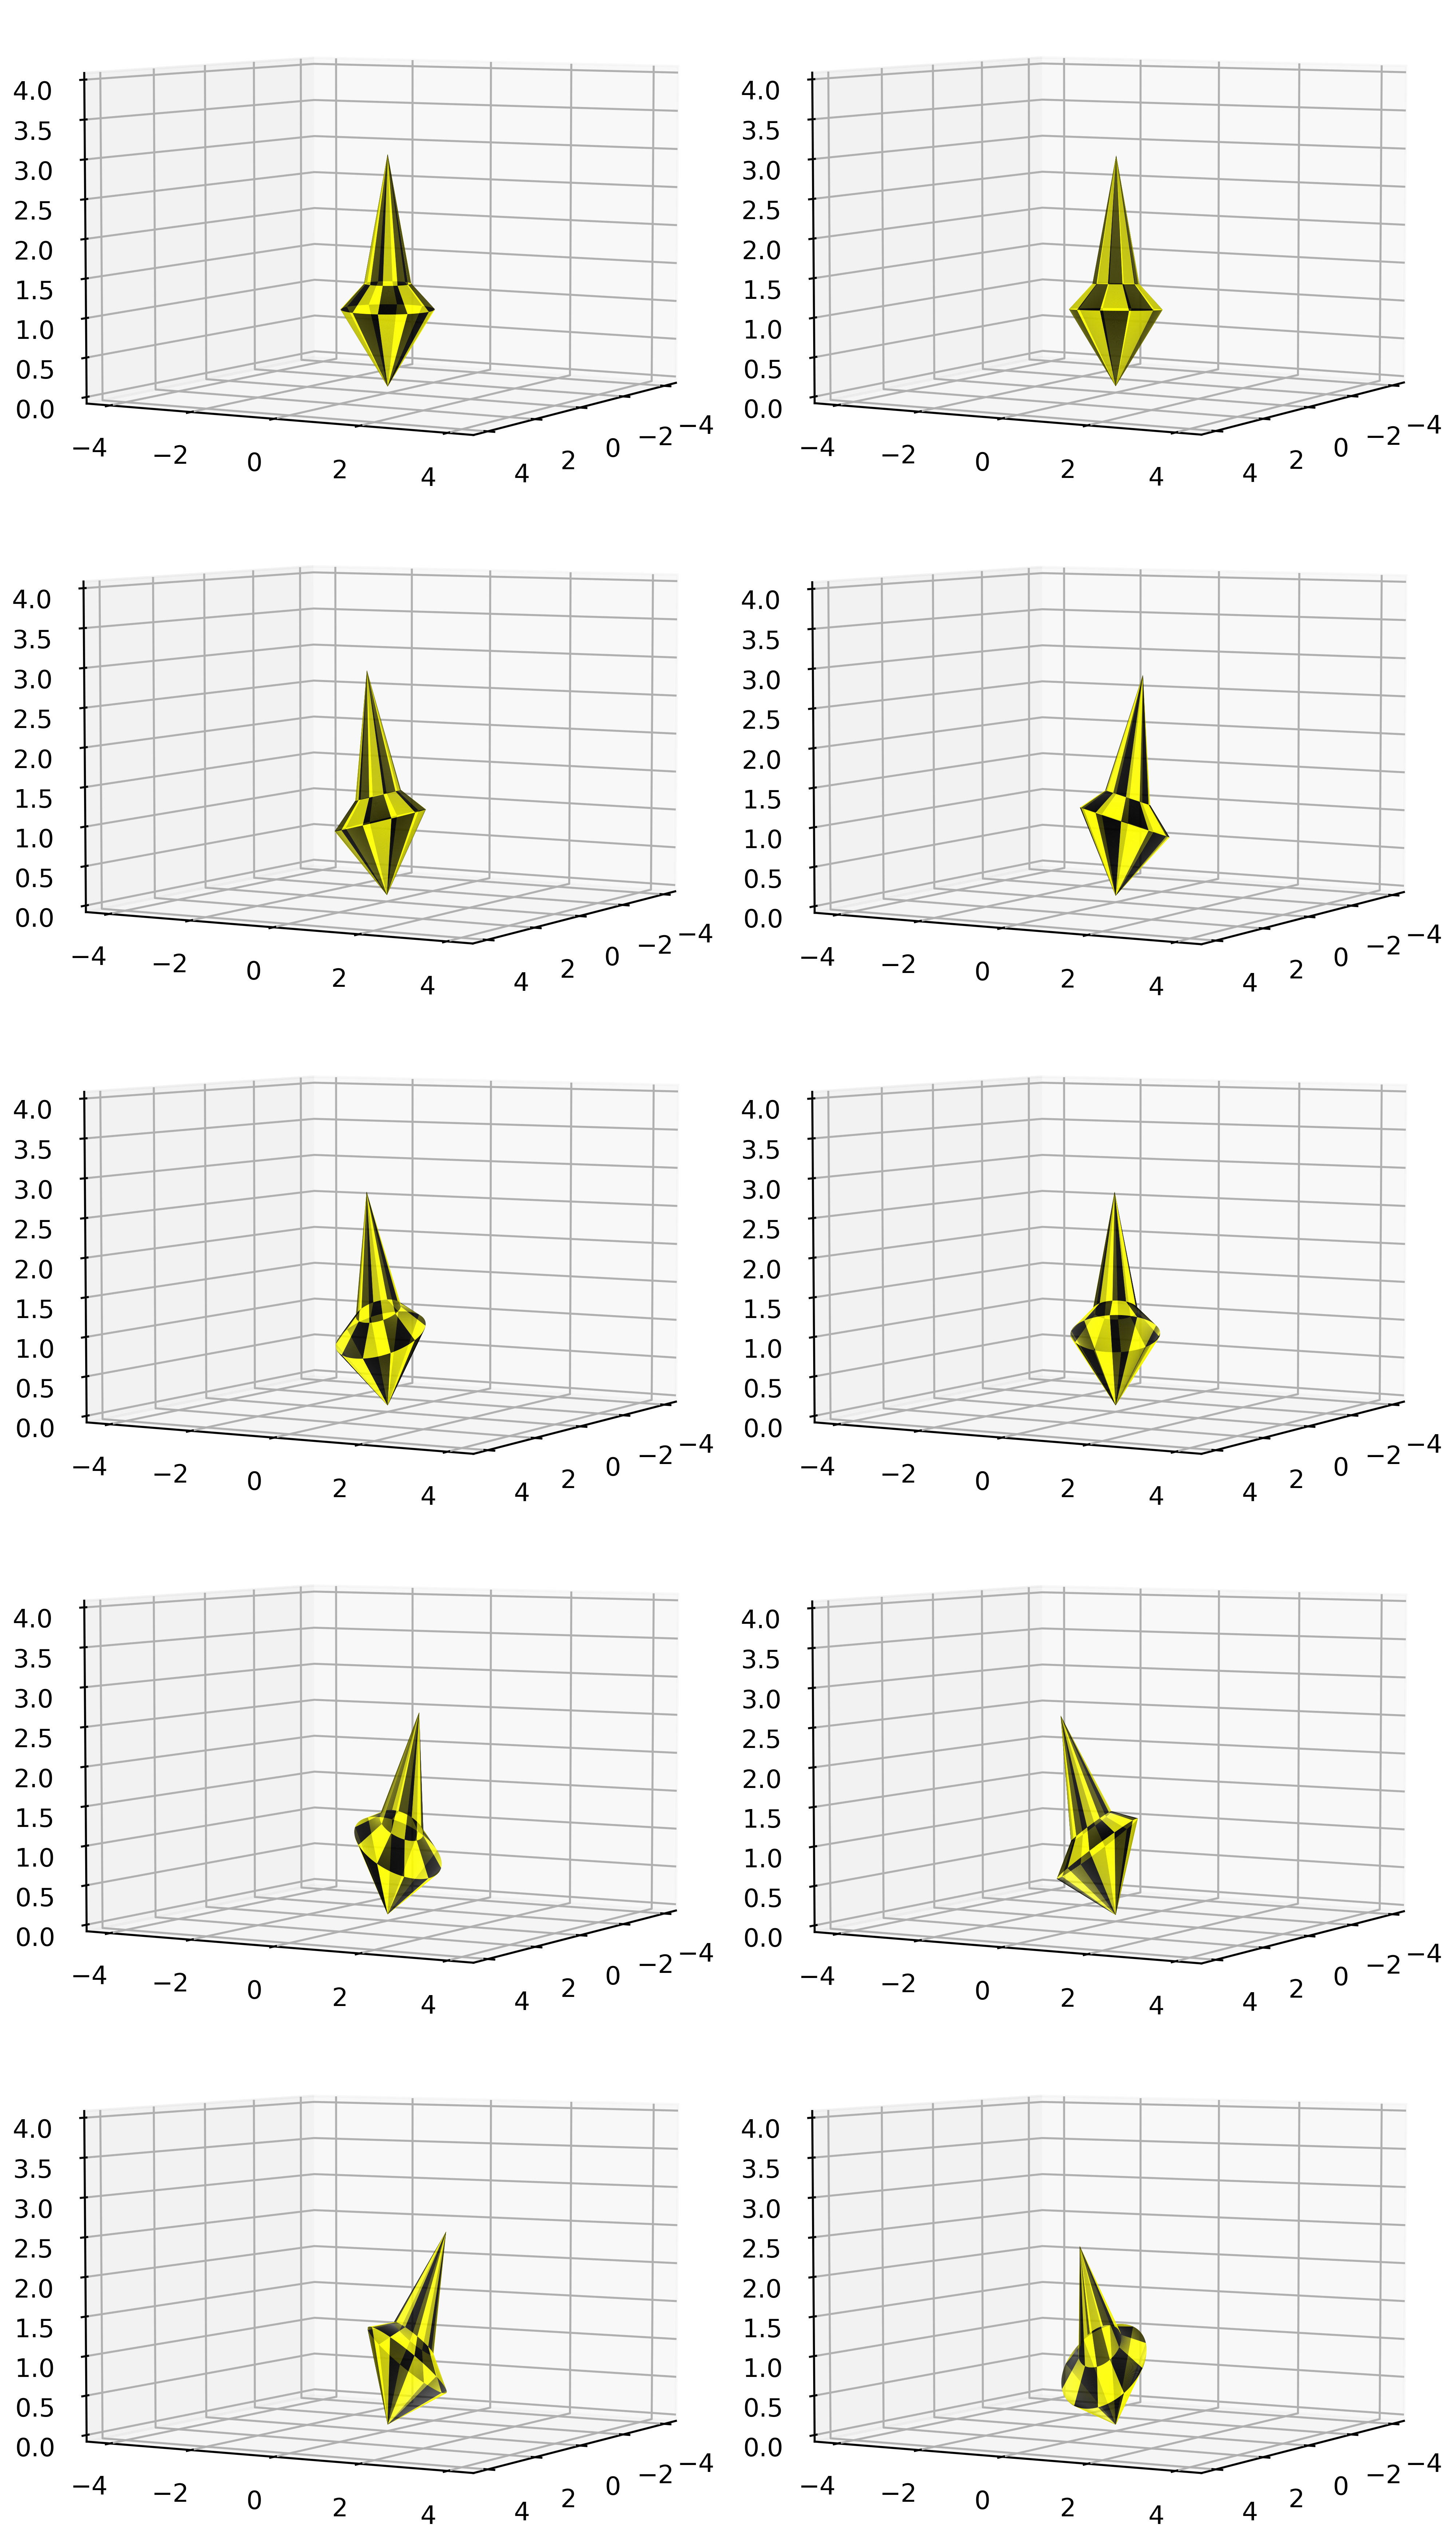
\includegraphics[width=14 cm]{Animation_pic.png}
\caption{Klatki oznaczone numerami (od lewej): $0,49,99,149,199,249,299,349,399,449$ oraz $499$}
\end{center}
\end{figure}

\subsection{Animacja w przy użyciu obrotu macierzowego}

\chapter{Literatura}
\end{document}